% **************************************************
% Document Class Definition
% **************************************************
\documentclass[%
    paper=A4,               % paper size --> A4 is default in Germany
    twoside=true,           % onesite or twoside printing
    openright,              % doublepage cleaning ends up right side
    parskip=half,           % spacing value / method for paragraphs
    chapterprefix=true,     % prefix for chapter marks
    11pt,                   % font size
    headings=normal,        % size of headings
    bibliography=totoc,     % include bib in toc
    listof=totoc,           % include listof entries in toc
    titlepage=on,           % own page for each title page
    captions=tableabove,    % display table captions above the float env
    chapterprefix=false,    % do not display a prefix for chapters
    appendixprefix=false,    % but display a prefix for appendix chapter
    draft=false,            % value for draft version
]{scrreprt}%


% **************************************************
% Setup YOUR thesis document in this file !
% **************************************************
% !TEX root = my-thesis.tex


% **************************************************
% Files' Character Encoding
% **************************************************
\PassOptionsToPackage{utf8}{inputenc}
\usepackage{inputenc}


% **************************************************
% Information and Commands for Reuse
% **************************************************
\newcommand{\thesisTitle}{Answering Causal Questions \texorpdfstring{\\}{} with Reinforcement Learning}
\newcommand{\thesisName}{Lukas Blübaum}
\newcommand{\thesisSubject}{Master's Thesis}
\newcommand{\thesisDate}{\today}
\newcommand{\thesisVersion}{Final}

\newcommand{\thesisFirstReviewer}{Prof. Dr. Axel-Cyrille Ngonga Ngomo}
\newcommand{\thesisFirstReviewerUniversity}{\protect{Paderborn University}}
\newcommand{\thesisFirstReviewerDepartment}{Department of Computer Science}

\newcommand{\thesisSecondReviewer}{Jun.-Prof. Dr. Sebastian Peitz}
\newcommand{\thesisSecondReviewerUniversity}{\protect{Paderborn University}}
\newcommand{\thesisSecondReviewerDepartment}{Department of Computer Science}

\newcommand{\thesisFirstSupervisor}{Dr. Stefan Heindorf}
%\newcommand{\thesisSecondSupervisor}{John Smith}

\newcommand{\thesisUniversity}{\protect{Paderborn University}}
\newcommand{\thesisUniversityDepartment}{Faculty for Computer Science, Electrical Engineering and Mathematics}
\newcommand{\thesisUniversityInstitute}{Department of Computer Science}
\newcommand{\thesisUniversityGroup}{DICE Research Group}
\newcommand{\thesisUniversityCity}{Paderborn}
\newcommand{\thesisUniversityStreetAddress}{Warburger Straße 100}
\newcommand{\thesisUniversityPostalCode}{33098}


% **************************************************
% Debug LaTeX Information
% **************************************************
%\listfiles


% **************************************************
% Load and Configure Packages
% **************************************************
\usepackage[english]{babel} % babel system, adjust the language of the content
\PassOptionsToPackage{% setup clean thesis style
    figuresep=colon,%
    hangfigurecaption=false,%
    hangsection=true,%
    hangsubsection=true,%
    sansserif=false,%
    configurelistings=true,%
    colorize=full,%
    colortheme=bluemagenta,%
    configurebiblatex=true,%
    bibsys=biber,%
    bibfile=bib-refs,%
    bibstyle=alphabetic,%
    bibsorting=nty,%
}{cleanthesis}
\usepackage{cleanthesis}

\hypersetup{% setup the hyperref-package options
    pdftitle={\thesisTitle},    %   - title (PDF meta)
    pdfsubject={\thesisSubject},%   - subject (PDF meta)
    pdfauthor={\thesisName},    %   - author (PDF meta)
    plainpages=false,           %   -
    colorlinks=false,           %   - colorize links?
    pdfborder={0 0 0},          %   -
    breaklinks=true,            %   - allow line break inside links
    bookmarksnumbered=true,     %
    bookmarksopen=true          %
}


% **************************************************
% OWN PACKAGES
% **************************************************

\usepackage{pgfgantt}

\usepackage{tikz}
\usetikzlibrary{shapes, arrows, arrows.meta, calc, positioning, matrix}
\usepackage{amsmath,amssymb}
\usepackage{tikz-uml}
\usepackage{booktabs}
\usepackage{svg}
\usepackage[linesnumbered]{algorithm2e}
\usepackage{pgfplots}
\pgfplotsset{compat = 1.3} 
\usepackage{mathtools}

\usepackage{xcolor}
\newcommand{\todo}[2][]{\textcolor{red}{TODO\@: #2}}




% **************************************************
% COLORS
% **************************************************

\definecolor{tab20darkblue}{HTML}{4e79a7}
\definecolor{tab20darkgreen}{HTML}{59a14f}
\definecolor{tab20darkred}{HTML}{e15759}
\definecolor{tab20darkorange}{HTML}{f28e2b}
\definecolor{tab20darkturquoise}{HTML}{499894}
\definecolor{tab20darkgray}{HTML}{79706e}
\definecolor{tab20darkbrown}{HTML}{9d7660}
\definecolor{tab20darkpurple}{HTML}{b07aa1}
\definecolor{tabl20lighgreen}{HTML}{8cd17d}
\definecolor{tab20lightblue}{HTML}{a0cbd8}


\definecolor{newgreen}{HTML}{148f77}
\definecolor{brass}{HTML}{E1C16E}


% **************************************************
% Document CONTENT
% **************************************************
\begin{document}

% uncomment the following command to fill up pages with
% whitespace instead of aligning the first and last lines
% of a page (see \raggedbottom vs. \flushbottom)
%\raggedbottom

% --------------------------
% rename document parts
% --------------------------
%\renewcaptionname{ngerman}{\figurename}{Abb.}
%\renewcaptionname{ngerman}{\tablename}{Tab.}
\renewcaptionname{english}{\figurename}{Fig.}
\renewcaptionname{english}{\tablename}{Tab.}

% --------------------------
% Front matter
% --------------------------
\pagenumbering{roman}			% roman page numbing (invisible for empty page style)
\pagestyle{empty}				% no header or footers
% !TEX root = my-thesis.tex
%
% ------------------------------------  --> cover title page
\begin{titlepage}
	\pdfbookmark[0]{Cover}{Cover}
	\flushright
	\hfill
	\vfill
	{\LARGE\thesisTitle \par}
	\rule[5pt]{\textwidth}{.4pt} \par
	{\Large\thesisName}
	\vfill
	\textit{\large\thesisDate} \\
	Version: \thesisVersion
\end{titlepage}


% ------------------------------------  --> main title page
\begin{titlepage}
	\pdfbookmark[0]{Titlepage}{Titlepage}
	\tgherosfont
	\centering

	%{\Large \thesisUniversity} \\[4mm]
	
\includegraphics[width=10cm]{figures/uni-logo} \\[2mm]
	\textsf{\thesisUniversityDepartment} \\
	\textsf{\thesisUniversityInstitute} \\
	\textsf{\thesisUniversityGroup} \\

	\vfill
	{\large \thesisSubject} \\[5mm]
	{\LARGE \color{ctcolortitle}\textbf{\thesisTitle} \\[10mm]}
	{\Large \thesisName} \\

	\vfill
	\begin{minipage}[t]{.27\textwidth}
		\raggedleft
		\textit{1. Reviewer}
	\end{minipage}
	\hspace*{15pt}
	\begin{minipage}[t]{.65\textwidth}
		{\Large \thesisFirstReviewer} \\
	  	{\small \thesisFirstReviewerDepartment} \\[-1mm]
		{\small \thesisFirstReviewerUniversity}
	\end{minipage} \\[5mm]
	\begin{minipage}[t]{.27\textwidth}
		\raggedleft
		\textit{2. Reviewer}
	\end{minipage}
	\hspace*{15pt}
	\begin{minipage}[t]{.65\textwidth}
		{\Large \thesisSecondReviewer} \\
	  	{\small \thesisSecondReviewerDepartment} \\[-1mm]
		{\small \thesisSecondReviewerUniversity}
	\end{minipage} \\[10mm]
	\begin{minipage}[t]{.27\textwidth}
		\raggedleft
		\textit{Supervisor}
	\end{minipage}
	\hspace*{15pt}
	\begin{minipage}[t]{.65\textwidth}
		\thesisFirstSupervisor\ %and \thesisSecondSupervisor
	\end{minipage} \\[10mm]

	\thesisDate \\

\end{titlepage}


% ------------------------------------  --> lower title back for single page layout
\hfill
\vfill
{
	\small
	\textbf{\thesisName} \\
	%\textit{\thesisTitle} \\
	\textit{Answering Causal Questions with Reinforcement Learning} \\
	\thesisSubject, \thesisDate \\
	Reviewers: \thesisFirstReviewer\ and \thesisSecondReviewer \\
	Supervisor: \thesisFirstSupervisor\ \\[1.5em]%and \thesisSecondSupervisor \\[1.5em]
	\textbf{\thesisUniversity} \\
	\textit{\thesisUniversityGroup} \\
	\thesisUniversityInstitute \\
	\thesisUniversityDepartment \\
	\thesisUniversityStreetAddress \\
	\thesisUniversityPostalCode\ \thesisUniversityCity
}
		% INCLUDE: all titlepages
\cleardoublepage

% This is the legal statement
%  - that your thesis is a work of your own,
%  - that you have not used any source other than the ones you mention, 
%  - that you genuinely created your theses to achieve the desired academic
%    degree, and have not presented it to another examination board; and
%  - that you have clearly marked all concepts and ideas that you have adopted
%    from other works.
\chapter*{Erklärung}
	\thispagestyle{empty}
	Ich versichere, dass ich die Arbeit ohne fremde Hilfe und ohne
	Benutzung anderer als der angegebenen Quellen angefertigt habe und dass
	die Arbeit in gleicher oder ähnlicher Form noch keiner anderen
	Prüfungsbehörde vorgelegen hat und von dieser als Teil einer
	Prüfungsleistung angenommen worden ist. Alle Ausführungen, die wörtlich
	oder sinngemäß übernommen worden sind, sind als solche
	gekennzeichnet.\\
	\vspace{27pt}

	\begin{center}
		\begin{tabular}{l p{0.1\textwidth} r}
			\cline{1-1} \cline{3-3}
			\begin{minipage}[t]{0.4\textwidth}
				\centering
				Ort, Datum
			\end{minipage}
			&&  
			\begin{minipage}[t]{0.4\textwidth}
				\centering
				Unterschrift
			\end{minipage}
	\end{tabular}
\end{center}


\cleardoublepage

%\vspace*{\fill}
\chapter*{Abstract}
Causal questions seek to determine whether there exists a causal relationship 
between different events or phenomena. 
Specifically, they often aim to understand the underlying causes of an effect or what kind of effects a particular cause might have in the future.
Causal questions are important for various use cases, for example, in virtual assistants or search engines.
However, many current approaches to causal question answering cannot provide explanations or verifications for their answers. 
Additionally, the approaches were often missing 
large-scale datasets of causal relations.
In this thesis, we explore the application of reinforcement learning on CauseNet, a large-scale causal knowledge graph, to answer binary causal questions inspired by the successful application of reinforcement learning in knowledge graph tasks, such as link prediction and fact-checking.
We introduce an Actor-Critic based agent which learns to search through the graph to answer binary causal questions.
Additionally, we bootstrap the agent with a supervised learning procedure and adapt an existing reward shaping strategy to deal 
with large action spaces and sparse rewards.
Our evaluation shows that our agent successfully prunes the search to answer binary causal questions efficiently.
Moreover, our ablation study indicates that the supervised learning strategy provides a strong foundation upon which the agent can improve.
Finally, we demonstrate how the paths learned by the agent can be used to explain causal relations, to indicate the specific mechanisms by which a cause produces an effect.
%\vspace*{\fill}
\cleardoublepage

%\emptypage

\pagestyle{plain}				% display just page numbers
%%\vspace*{\fill}
\chapter*{Abstract}
Causal questions seek to determine whether there exists a causal relationship 
between different events or phenomena. 
Specifically, they often aim to understand the underlying causes of an effect or what kind of effects a particular cause might have in the future.
Causal questions are important for various use cases, for example, in virtual assistants or search engines.
However, many current approaches to causal question answering cannot provide explanations or verifications for their answers. 
Additionally, the approaches were often missing 
large-scale datasets of causal relations.
In this thesis, we explore the application of reinforcement learning on CauseNet, a large-scale causal knowledge graph, to answer binary causal questions inspired by the successful application of reinforcement learning in knowledge graph tasks, such as link prediction and fact-checking.
We introduce an Actor-Critic based agent which learns to search through the graph to answer binary causal questions.
Additionally, we bootstrap the agent with a supervised learning procedure and adapt an existing reward shaping strategy to deal 
with large action spaces and sparse rewards.
Our evaluation shows that our agent successfully prunes the search to answer binary causal questions efficiently.
Moreover, our ablation study indicates that the supervised learning strategy provides a strong foundation upon which the agent can improve.
Finally, we demonstrate how the paths learned by the agent can be used to explain causal relations, to indicate the specific mechanisms by which a cause produces an effect.
%\vspace*{\fill}		% INCLUDE: the abstracts (english and german)
\cleardoublepage
%
%\input{content/acknowledgement} % INCLUDE: acknowledgement
\cleardoublepage
%
\currentpdfbookmark{\contentsname}{toc}
\setcounter{tocdepth}{2}		% define depth of toc
\tableofcontents				% display table of contents
\cleardoublepage

% --------------------------
% Body matter
% --------------------------
\pagenumbering{arabic}			% arabic page numbering
\setcounter{page}{1}			% set page counter
\pagestyle{scrheadings}			% header and footer style

%% Uncomment the following lines using the \part command
%% to add part sections
% !TEX root = my-thesis.tex
%
\chapter{Introduction}
\label{ch:introduction}

Causal question answering addresses the problem of determining the causal relations between given causes and effects~\cite{KayeshCausalTransfer2020, DalalCausalQAEnhancing2021}. This could involve examining whether a causal relation exists or how a causal relation can be explained.
For example, causal questions like \textit{``Does pneumonia cause anemia?''} ask for the validity of a causal relation.
Instead, more complicated questions like \textit{``How does pneumonia cause death?''} might ask for an explanation of a causal relation. 
Nowadays, the necessity to answer causal questions arises in various domains. For example, users often seek answers to causal questions from virtual assistants like Alexa or from search engines~\cite{Nguyen2016MSMARCO, Heindorf2020Causenet}. Similarly, causal questions and explanations for causal relations are important for argumentation~\cite{Walton2007Dialog, Habernal2018Argumentation} and automated decision-making~\cite{HassanzadeshCausalQA2019, KayeshCausalTransfer2020, Heindorf2020Causenet}.
When possible, tracing the causality chain that led to an answer can provide further insights and a deeper understanding of the causal relationship in question.


%\begin{itemize}
%    \item example
    %\item learned by humans through everyday life, still often not true or justified (CauseNet paper)
    %\item maybe historic context, aristotle, socrates
    %\item Important because many causal questions (asked by search engine users, c.f., MS MARCO), alexa, necessary for argumentation, decision making
    %\item judea pearl, the book of why -- correlation -> causality
%\end{itemize}


Therefore, the literature started to introduce approaches for causal question answering~\cite{SharpCausalQAEmbeddings2016, HassanzadeshCausalQA2019, KayeshCausalTransfer2020, DalalCausalQAISWC2021}. 
Some approaches focus on binary questions~\cite{HassanzadeshCausalQA2019, KayeshCausalTransfer2020}, 
while others extend the setting to multiple-choice questions~\cite{SharpCausalQAEmbeddings2016, DalalCausalQAISWC2021}.
However, a limitation of most of these approaches is the lack of explanations or verifiability of their answers. 
Additionally, they identified the problem of a lack of large, high-quality datasets for causal relations~\cite{SharpCausalQAEmbeddings2016, HassanzadeshCausalQA2019, KayeshCausalTransfer2020}. 
Consequently, the authors resorted to creating their own datasets from sources like news articles or Wikipedia to support the identification of causal relations to answer causal questions. 
Thus, the introduction of CauseNet~\cite{Heindorf2020Causenet}, a large-scale knowledge graph consisting of causal relations with context information, provides new opportunities to build effective causal question answering systems. 
Accordingly, we can apply various approaches from the knowledge graph literature that utilize the structure and rich semantics.

In particular, reinforcement learning was successfully applied to knowledge graphs on different tasks such as link prediction~\cite{Xiong2017DeePpath}, 
fact-checking~\cite{Das2018Minerva}, or conversational question answering~\cite{Kaiser2021Reinforcement}. 
In this thesis, we explore whether we can model the
causal question answering task as a sequential decision problem similar to the aforementioned approaches.
Our initial focus is on binary causal questions, with the potential for extension to open-ended questions in future works.
We train a reinforcement learning agent that learns to walk over CauseNet to find good inference paths to answer binary causal questions.
 The resulting reasoning capabilities are beneficial for questions whose answers require a chain of multiple hops~\cite{Xiong2017DeePpath, Das2018Minerva, Wan2021GaussianPath}. 

We implemented the agent via the Synchronous Advantage Actor-Critic (A2C) algorithm~\cite{Mnih2016A2C} and used 
generalized advantage estimation (GAE)~\cite{Schulman2016GAE} to compute the advantage. 
To address the challenge of a large action space in CauseNet~\cite{Heindorf2020Causenet}, we bootstrap the agent with a supervised learning procedure at the start~\cite{Xiong2017DeePpath}.
During the supervised learning, the agent receives expert demonstrations to understand what good paths look like.
To handle sparse rewards during training, we enhance 
the agent with a reward shaping technique based on prior works~\cite{Yasunaga2021QAGNN}.
Our evaluation demonstrates that the agent can effectively prune the search space, considering only a small number of nodes for each question. 
Additionally, our experiments confirm that the supervised learning phase establishes a strong foundation for the agent, decreasing the uncertainty in identifying good paths and accelerating the learning process. 
Moreover, we demonstrate how paths found by our agent can be used to explain the relations between a given cause and effect, including the option to take the original source into account~\cite{Heindorf2020Causenet}.
Furthermore, we discuss straightforward options to extend our approach to different causal question types.
% OLD
%Using this approach, the agent is able to answer binary questions or questions that ask for a simple cause or effect. 
%However, it might be hard to answer complex questions which expect more detailed answers. Consequently, for these question types, we propose to take the paths extracted by the agent and feed them into a pre-trained language model~\cite{Vaswani2017Attention, Khashabi2020UnifiedQA} as additional context. 
%Dalal et al.~\cite{DalalCausalQAEnhancing2021, DalalCausalQAISWC2021} already consider a similar setup applied on CauseNet. However, they extract relevant causal relations via string matching while we use the paths found by the RL agent. Notably, the paths that led to an answer allow for post-hoc explanations and enable the user to follow the reasoning chain. In case of CauseNet~\cite{Heindorf2020Causenet}, we can also take the context information into account. Thus, for each relation on a path, we can provide supplemental explanations such as the original sentences and source URLs.

To summarize, our contributions are:
\begin{enumerate}
    \item We introduce the first reinforcement learning approach for causal question answering on knowledge graphs.
    \item We implemented an agent with the Synchronous Advantage Actor-Critic (A2C) algorithm, including a supervised learning procedure and a 
        reward shaping technique to handle the challenges of the large action space and sparse rewards.
    \item We extend an existing approach for extracting binary causal questions and introduce a new binary causal question dataset.
\end{enumerate}


Overall, this thesis is structured as follows. First, we introduce related work in Chapter~\ref{ch:related-work}. 
Next, we present preliminaries discussing key methods and ideas our approach relies upon in Chapter~\ref{sec:preliminaries}. In Chapter~\ref{ch:approach}, we introduce our approach in detail, and in Chapter~\ref{ch:implementation}, we discuss our implementation.
Chapter~\ref{ch:evaluation} evaluates our approach, including an ablation study. Finally, we discuss some findings and future work in Chapter~\ref{ch:discussion}, followed by the conclusion in Chapter~\ref{ch:conclusion}.

   % INCLUDE: introduction
% !TEX root = proposal.tex
%
\chapter{Related Work}
\label{sec:related}

In the following, we summarize related work. First, we
provide an overview of approaches for causal question answering. These approaches mainly employ pattern-based searches, embeddings, and language models. To the best of our knowledge, we are the first to use reinforcement learning for causal question answering. Afterward, we present several knowledge graphs that focus on causal and commonsense knowledge. Lastly, we discuss approaches that apply reinforcement learning to reasoning and question answering tasks on knowledge graphs.
\paragraph{Causal Question Answering}

Currently, only few approaches directly focus on the causal question answering task. Most of these approaches focus on binary questions, i.e., questions such as ``\textit{Does X cause Y?}'' which expect a yes or no answer. 
Kayesh et al.~\cite{KayeshCausalTransfer2020} model the task as a transfer learning approach. Therefore, they extract cause-effect pairs from news articles via causal cue words. Subsequently, they transform the pairs into sentences of the form ``\textit{X may cause Y}'' and use them to finetune BERT~\cite{DevlinBert2019}. Similarly, Hassanzadesh et al. \cite{HassanzadeshCausalQA2019} employ large-scale text mining to answer binary causal questions. They introduce several unsupervised approaches ranging from simple string matching to embeddings computed via BERT. Each approach uses the text corpora to find evidence for a potential causal relation. Afterward, the evidence is used to compute a score that results in a yes or no answer depending on a threshold value.


Instead, Sharp et al.~\cite{SharpCausalQAEmbeddings2016} consider multiple-choice questions of the form ``\textit{What causes X?}''. First, they mine cause-effect pairs from Wikipedia via syntactic patterns and train an embedding model to capture the semantics between the pairs. At inference time, they compute the embedding similarity between the question and each answer candidate. The approach by Dalal et al.~\cite{DalalCausalQAEnhancing2021, DalalCausalQAISWC2021} is most similar to ours.
Given a question, they apply string matching to extract relevant causal relations from CauseNet~\cite{Heindorf2020Causenet}. Subsequently, they provide the question with the causal relations to a language model as additional context. In our work, we consider a similar idea for complex questions by selecting relevant paths via a reinforcement learning agent.

Another approach that combines knowledge graphs and language models is QA-GNN~\cite{Yasunaga2021QAGNN}.
Specifically, QA-GNN creates an augmented graph by scoring entities and relations with a pre-trained language model according to their relevance to the question. Then, QA-GNN applies a graph attention network (GAT)~\cite{Velickovic2018GAT} on the augmented graph to answer the question. Likewise, we apply the RL agent on an augmented graph to provide a better reward signal, similar to the reward shaping strategies by prior RL approaches on knowledge graphs~\cite{Lin2020RewardShaping, Qiu2020Stepwise}.


%\cite{Lu2019ComplexSteiner} Build a quasi KG from text documents which contain entities and phrases relevant to the question. Assign weights to nodes and edges. Find answers by solving a Group Steiner Tree problem~\cite{ReichSteiner1989} on the created quasi KG. 

\paragraph{Causal Knowledge Graphs}
ConceptNet~\cite{Speer2017ConceptNet} is a general knowledge graph consisting of relations between natural language terms, which contains 36 relations, including a \textit{Causes} relation. CauseNet~\cite{Heindorf2020Causenet} and Cause Effect Graph~\cite{Li2020CauseEffectGraph} take a narrower view and specifically focus on causal relations extracted via linguistic patterns from web sources like Wikipedia and ClueWeb12~\footnote{https://lemurproject.org/clueweb12/}. 

In contrast, ATOMIC~\cite{Sap2019ATOMIC} focuses on inferential knowledge. Specifically, ATOMIC consists of \textit{``If-Event-Then-X''} relations that are based on social interactions or events in the real world. ATOMIC$^{20}_{20}$~\cite{Hwang2021COMET} selects relations from ATOMIC and ConceptNet to create an improved graph while adding more relations via crowdsourcing. Instead, West et al.~\cite{West2021Symbolic} automate the curation of inferential relations by clever prompting of a language model. Finally, CSKG~\cite{Ilievski2021CSKG} builds a consolidated graph combining seven knowledge graphs, including ConceptNet and ATOMIC.
For this thesis, we focus on CauseNet and potentially Cause Effect Graph because most of the other knowledge graphs either focus on inferential knowledge or are not limited to causal relations. Although, if time permits, making use of a combination of multiple graphs might be a potential improvement.

\paragraph{Knowledge Graph Reasoning with Reinforcement Learning}

In recent years, reinforcement learning on knowledge graphs has been applied in link prediction~\cite{Das2018Minerva}, fact checking~\cite{Xiong2017DeePpath}, or question answering~\cite{Qiu2020Stepwise}. Given a source and a target entity, DeepPath~\cite{Xiong2017DeePpath} learns to find paths between them. In the first step, DeepPath is trained in a supervised manner on paths found by BFS. Afterward, DeepPath applies REINFORCE~\cite{Williams1992REINFORCE} policy gradients to improve the policy further.
During inference time, the paths are used to predict links between entities or check the validity of triples. Subsequently, MINERVA~\cite{Das2018Minerva} improves on DeepPath by introducing an LSTM~\cite{Hochreiter1997LSTM} into the policy network to account for the path history. Moreover, MINERVA does not require knowledge of the target entity and is trained end-to-end without supervision at the start. Lin et al.~\cite{Lin2020RewardShaping} propose two improvements for MINERVA. First, they apply reward shaping by scoring the paths with a pre-trained KG embedding model~\cite{Dettmers2018ConvE} to reduce the problem of sparse rewards. Second, they introduce a technique called action dropout, which randomly disables edges at each step. Action dropout serves as additional regularization and helps the agent learn diverse paths.


Contrary to these approaches, M-Walk~\cite{Shen2018MWalk} does not rely on REINFORCE but instead looks at the problem from a model-based viewpoint. 
Like AlphaZero~\cite{Silver2018AlphaZero}, M-Walk applies Monte Carlo Tree Search (MCTS) as a policy improvement operator. Thus, at each step, M-Walk applies MCTS to produce trajectories of an improved policy and subsequently trains the current policy to imitate the improved one. GaussianPath~\cite{Wan2021GaussianPath} takes a Bayesian view of the problem and represents each entity by a gaussian distribution to better model uncertainty.

While all these approaches focus on link prediction or fact checking, there has been some work on natural language question answering.
Qiu et al.~\cite{Qiu2020Stepwise} introduce the Stepwise Reasoning Network (SRN).
They observe that for questions requiring multiple hops, different parts of the question should be important at each time step. Therefore, they introduce an attention mechanism into the policy network to enable the agent to attend to different parts of the question at every step. In turn, this should help the agent to focus on the aspect of the question that is important for the current decision. Additionally, SRN utilizes extra reward signals by considering the semantic similarities between the question and the action history via a potential-based reward function~\cite{Ng1999Potential}. CONQUER~\cite{Kaiser2021Reinforcement} employs REINFORCE policy gradients for conversational question answering. Multiple agents search through the graph in parallel and aggregate their answers at the end. Importantly, the reward depends on user feedback. A positive reward corresponds to a new question, and a negative reward to a reformulation of the last question.


%\begin{itemize}
%    \item Variational Reasoning for Question Answering with Knowledge Graph
%    \item Anytime Bottom-Up Rule Learning for Knowledge Graph Completion
%    \item Safran: https://arxiv.org/pdf/2109.08002.pdf
%\end{itemize}




%\textbf{https://github.com/THU-KEG/Knowledge\_Graph\_Reasoning\_Papers}   % INCLUDE: related work

% !TEX root = my-thesis.tex
%
\chapter{Preliminaries}
\label{sec:preliminaries}

To start with, we provide an overview of the key concepts and methods 
our approach relies on. 
First, we discuss the causal knowledge graph CauseNet~\cite{Heindorf2020Causenet} in more detail. 
Next, we examine different types of causal 
questions and discuss the process of curating our causal question dataset. 
Finally, we provide a brief introduction to reinforcement learning, 
including the REINFORCE~\cite{Williams1992REINFORCE} and Synchronous Advantage Actor-Critic (A2C)~\cite{Mnih2016A2C} algorithms.

\section{CauseNet}
\label{subsec:causal-kgs}
CauseNet~\cite{Heindorf2020Causenet} is a large-scale causal knowledge graph of causal relations.
Specifically, CauseNet contains \textit{claimed} causal relations because they were extracted 
from web sources like Wikipedia and ClueWeb12\footnote{\url{https://lemurproject.org/clueweb12/}} that are not necessarily true.
Formally, CauseNet is defined as $\mathcal{K} = (\mathcal{E}, \mathcal{R})$, where 
$\mathcal{E}$ represents the set of entities and $\mathcal{R}$ is the set of relations. 
The entities in CauseNet are single words or noun phrases, while the set of relations 
contains only the \textit{mayCause} relation, i.e., $\mathcal{R} = \{mayCause\}$.\footnote{In this thesis we will use \textit{cause} when talking about the relations.}
Figure~\ref{fig:graph_example} shows an excerpt from CauseNet. It shows the entity \textit{pneumonia} together 
with some of its causes and effects. The causal relations are stored as triples, e.g., 
$(pneumonia, mayCause, sepsis) \in \mathcal{K}$ where $pneumonia, sepsis \in \mathcal{E}$.
Moreover, CauseNet contains additional meta-information for each relation.
Included are the original source, i.e., the URL of the web page and the original sentence,
if applicable.

%The causal relations were extracted from Wikipedia and 
%First, they defined a set of established causal relations containing a cause and an effect, e.g., 
%\textit{smoking} and \textit{cancer}.
%Next, they searched for sentences that contain the cause and effect of one relation and extracted linguistic patterns from the sentences.
%Consequently, the linguistic pattern can be used to find further causal relations.
CauseNet has two configurations, a high-precision one (CauseNet-Precision) and a high-recall one (CauseNet-Full).
The statistics of both graphs can be seen in Table~\ref{table-causenet}.
%CauseNet-Full contains all extracted relations, while CauseNet-Precision
%only contains relations that were extracted by patterns
%which received a support of atleast two. Heindorf et al.~\cite{Heindorf2020Causenet} defined the support of a pattern by the number of seeds 
%which made use of the pattern.
CauseNet-Precision contains around 2\% of the original relations, increasing 
the precision from 83\% to 96\%. The precision was evaluated by randomly selecting 
a number of relations from the graphs and manually evaluating them for correctness.

\begin{table}
\caption{The statistics of CauseNet-Full and CauseNet-Precision, including their precision,
the number of entities, and the number of relations. The numbers were taken from the paper~\cite{Heindorf2020Causenet}.}
\label{table-causenet}
\centering
\begin{tabular}{lrrr} 
			\toprule
			\textbf{Graph} & \textbf{Precision} & \textbf{|Concepts/Entities|} & \textbf{|Relations|}\\
			\toprule
		   CauseNet-Full & 83\% & 12,186,31& 11,609,89 \\
		   CauseNet-Precision & 96\% & 80,223 &	197,806\\
			\bottomrule
\end{tabular}
\end{table}

\section{Causal Questions}
\label{subsec:causal-questions}

Causal questions seek to determine whether there exists a causal relationship 
between different events or phenomena. Often, their goal is to understand why something 
happened or to predict what kind of effects a certain cause might have in the future.

Generally, we can differentiate between different types of causal questions.
Starting with simple binary questions that ask for the validity of a 
causal relation, such as \textit{``Does smoking cause cancer?''}. Another type are 
Cause-Effect questions which seek to identify the cause of a given effect or vice versa.
An example of this type of question is \textit{``What causes the rise in global temperatures?''}.
Additionally, there are more complex questions that investigate the relationship between multiple entities.
For example, a question like \textit{``How does smoking cause cancer?''} examines the specific mechanisms by which the cause produces the effect.
For the first version of our approach, we only consider binary causal questions like 
many prior approaches~\cite{HassanzadeshCausalQA2019, KayeshCausalTransfer2020}.
However, we discuss a simple extension to Cause-Effect questions in Chapter~\ref{ch:discussion}
for future work.

To construct a dataset of binary causal questions, we extracted them from the Webis-CausalQA-22 corpus~\cite{Bondarenko2022CausalQA}.\footnote{\url{https://zenodo.org/record/7476615}}
CausalQA is a corpus for causal question answering containing around 1.1 million
causal questions. The corpus was constructed by extracting causal questions from ten
well-known question answering datasets, such as SQuAD v2.0~\cite{rajpurkar:2018} and MS MARCO~\cite{nguyen:2016}.
For a full list of the datasets, including their references, see Table~\ref{table-causal-datasets}.
The table also shows the number of total causal questions and the number of binary 
causal questions that we extracted for each dataset. After the extraction, only
MS MARCO contains a sufficient number of binary causal questions for use in our experiments.
The scarcity of binary causal questions in the datasets may be due to a number of reasons. One factor is that many datasets, 
such as NewsQA~\cite{trischler:2017} and HotpotQA~\cite{yang:2018}, have a limited number of causal questions to begin with.
Additionally, some larger datasets like ELI5~\cite{fan:2019} are focused on open-ended question
 answering.


\begin{table}
\caption{A few binary causal questions that we extracted from the datasets. The 
cause of each question is colored in \textcolor{tab20darkgreen}{green}, and the effect in \textcolor{tab20darkblue}{blue}.}
\label{table-example-questions}
	\centering
\begin{tabular}{lc}
	\toprule
	\textbf{Question} & \textbf{Answer}\\
	\midrule
	Can \textcolor{tab20darkgreen}{alcohol} cause \textcolor{tab20darkblue}{diabetes}? & Yes \\
	Will \textcolor{tab20darkgreen}{hot weather} affect \textcolor{tab20darkblue}{blood sugar}? & Yes \\
	Is \textcolor{tab20darkblue}{malaria} caused by a \textcolor{tab20darkgreen}{fungus}? & No \\
	Does \textcolor{tab20darkgreen}{depo provera} cause \textcolor{tab20darkblue}{cancer}? & No \\
	\bottomrule
\end{tabular}
\end{table}

\newcommand{\pattern}[1]{\texttt{\fontsize{9.5pt}{10pt}\selectfont [#1]}\xspace}
For the extraction of binary causal questions, we built on work by 
Heindorf et al.~\cite{Heindorf2020Causenet} from CauseNet.
For their evaluation, they implemented an extraction mechanism for binary causal questions.
Specifically, the questions were extracted via patterns of the following form:
\begin{center}
\texttt{\selectfont [question word]\xspace}
\texttt{\selectfont [cause/effect]\xspace}
\texttt{\selectfont [causal cue word]\xspace}
\texttt{\selectfont [cause/effect]\xspace} ?
\end{center}
where the \texttt{\selectfont [question word]\xspace} placeholder either represents one of the question words from 
Table~\ref{table-questions-pos-tags} or is empty. The \texttt{\selectfont [causal cue word]\xspace} placeholder 
represents words that are good indicators for causal relations together with their appropriate prepositions. Therefore, they should 
identify whether a question is causal or not. The original approach
only considered \textit{cause} in different verb forms, e.g., infinitive, past, or progressive.
We extended this to consider a greater number of causal cue words.
Specifically, we used the collection from Girju et al.~\cite{Girju2002CausalCue}.
Girju et al. curated a collection of causal cue words and ranked them by their 
frequency and ambiguity, i.e., how often they appear in text and how often they 
refer to a causal relation. 
Among these, we selected the ones that were ranked with high frequency and low 
ambiguity.
Table~\ref{table-cue-words} shows the full list of 23 words. 

Moreover, the \texttt{\selectfont [cause/effect]\xspace} placeholder 
represents causal concepts, where one takes the role of the cause and the other 
the role of the effect. The order depends on the question word and the causal cue word. Like
 Heindorf et al.~\cite{Heindorf2020Causenet}, we place a few restrictions 
on the questions to keep the causal concepts simpler. This should increase 
the probability that the concepts can be found in CauseNet because we can only 
use questions where both the cause and effect can be found. The restrictions are 
enforced by filtering questions on a number of POS-Tags from the Stanford CoreNLP~\cite{Manning2014NLP}.
The full list is shown in Table~\ref{table-questions-pos-tags} on the right.
Among others, we disallow coordinating conjunctions or subordinating conjunctions.
Finally, we check whether the questions are answered with ``yes'' or ``no'' and remove 
any further explanation. Table~\ref{table-example-questions} shows a few questions which 
we extracted from the datasets.

To summarize, the extraction focuses on binary causal questions that contain 
exactly one cause and one effect identified by one of 23 causal cue words.

%\begin{table}
\centering
\caption{The ten datasets that are part of CausalQA~\cite{Bondarenko2022CausalQA}. The
		\textit{Total} column shows the total number of causal questions for each dataset, 
		while the \textit{Binary} column shows the number of binary causal questions.
		Note that the test sets are either not publically available or 
		are missing the answers.}
\label{table-causal-datasets}
	\begin{tabular}{lrrrrr} 
		\toprule
		\textbf{Dataset} & \multicolumn{2}{c}{\textbf{Total}} & \multicolumn{2}{c}{\textbf{Binary}} & \textbf{Reference} \\
		\cmidrule(lr{.6em}){2-3} \cmidrule(l{0.4em}){4-5}
		&\textbf{|Train|} & \textbf{|Valid|} & \textbf{|Train|} & \textbf{|Valid|} & \\
		\midrule
		PAQ & 692,645 & 76,961 & 1 & --  & \cite{Lewis2021PAQ}\\ 
		GooAQ & 146,253 & 33 & 167 & -- &  \cite{khashabi:2021}\\
		MS MARCO & 41,764 & 2,558 & 2,410 & 263 & \cite{nguyen:2016} \\
		Natural Questions & 2,796 & 71 & -- & -- & \cite{kwiatkowski:2019}\\
		ELI5 & 131,035 & 4,834 & 2 & --  & \cite{fan:2019}\\
		SearchQA &663 & 117 & -- & -- & \cite{dunn:2017}\\
		SQuAD v2.0 & 4,342 & 483 & -- & -- & \cite{rajpurkar:2018}\\
		NewsQA &1,303 & 62 & -- & -- & \cite{trischler:2017}\\
		HotpotQA &355& 35 & -- & -- & \cite{yang:2018}\\
		TriviaQA & 637 & 66 & -- & -- & \cite{joshi:2017} \\
		\bottomrule
	\end{tabular}
\end{table}
\begin{table}
\caption{The causal cue words we used to detect binary causal questions. The list was
		curated by Girju et al.~\cite{Girju2002CausalCue} to include words that are 
		good indicators for causal relations, meaning they should have low ambiguity and high frequency.}
\label{table-cue-words}
\centering
	\begin{tabular}{rrrr}
	\toprule
	\multicolumn{4}{c}{\textbf{Causal Cue Words}} \\
	\midrule
	induce & provoke & relate (to) & trigger off \\
	give rise (to) & arouse & link (to) & bring on \\
	produce & elicit & stem (from)& result (from)\\
	generate & lead (to)& originate & trigger\\
	effect & derive (from)& bring forth& cause \\
	bring about & associate (with)& lead up &\\
	\bottomrule
	\end{tabular}
\end{table}
\begin{table}
\caption{The left table shows the question words we used for the binary question
extraction. The right table shows the forbidden POS tags for the binary question extraction.}
\label{table-questions-pos-tags}
	\centering
	\begin{tabular}{rr}
		\toprule
		\multicolumn{2}{c}{\textbf{Question Words}} \\
		\midrule
		is & do\\
		can  & does\\
		might & did \\
		would & will \\
		could & are\\
		may \\
		\bottomrule
	\end{tabular}
	\quad
	\begin{tabular}{ll}
		\toprule
		\textbf{POS-Tag} & \textbf{Description}\\
		\midrule
		CC & Coordinating conjunction \\
		IN & Preposition or subordinating conjunction \\
		TO & To-prepositions \\
		WDT & Wh-determiner \\
		WP & Wh-pronoun \\
		WRB & Wh-adverb \\
		\bottomrule
	\end{tabular}
\end{table}
\begin{table}
\centering
\caption{The ten datasets that are part of CausalQA~\cite{Bondarenko2022CausalQA}. The
		\textit{Total} column shows the total number of causal questions for each dataset, 
		while the \textit{Binary} column shows the number of binary causal questions.
		Note that the test sets are either not publically available or 
		are missing the answers.}
\label{table-causal-datasets}
	\begin{tabular}{lrrrrr} 
		\toprule
		\textbf{Dataset} & \multicolumn{2}{c}{\textbf{Total}} & \multicolumn{2}{c}{\textbf{Binary}} & \textbf{Reference} \\
		\cmidrule(lr{.6em}){2-3} \cmidrule(l{0.4em}){4-5}
		&\textbf{|Train|} & \textbf{|Valid|} & \textbf{|Train|} & \textbf{|Valid|} & \\
		\midrule
		PAQ & 692,645 & 76,961 & 1 & --  & \cite{Lewis2021PAQ}\\ 
		GooAQ & 146,253 & 33 & 167 & -- &  \cite{khashabi:2021}\\
		MS MARCO & 41,764 & 2,558 & 2,410 & 263 & \cite{nguyen:2016} \\
		Natural Questions & 2,796 & 71 & -- & -- & \cite{kwiatkowski:2019}\\
		ELI5 & 131,035 & 4,834 & 2 & --  & \cite{fan:2019}\\
		SearchQA &663 & 117 & -- & -- & \cite{dunn:2017}\\
		SQuAD v2.0 & 4,342 & 483 & -- & -- & \cite{rajpurkar:2018}\\
		NewsQA &1,303 & 62 & -- & -- & \cite{trischler:2017}\\
		HotpotQA &355& 35 & -- & -- & \cite{yang:2018}\\
		TriviaQA & 637 & 66 & -- & -- & \cite{joshi:2017} \\
		\bottomrule
	\end{tabular}
\end{table}
\begin{table}
\caption{The left table shows the question words we used for the binary question
extraction. The right table shows the forbidden POS tags for the binary question extraction.}
\label{table-questions-pos-tags}
	\centering
	\begin{tabular}{rr}
		\toprule
		\multicolumn{2}{c}{\textbf{Question Words}} \\
		\midrule
		is & do\\
		can  & does\\
		might & did \\
		would & will \\
		could & are\\
		may \\
		\bottomrule
	\end{tabular}
	\quad
	\begin{tabular}{ll}
		\toprule
		\textbf{POS-Tag} & \textbf{Description}\\
		\midrule
		CC & Coordinating conjunction \\
		IN & Preposition or subordinating conjunction \\
		TO & To-prepositions \\
		WDT & Wh-determiner \\
		WP & Wh-pronoun \\
		WRB & Wh-adverb \\
		\bottomrule
	\end{tabular}
\end{table}
\begin{table}
\caption{The causal cue words we used to detect binary causal questions. The list was
		curated by Girju et al.~\cite{Girju2002CausalCue} to include words that are 
		good indicators for causal relations, meaning they should have low ambiguity and high frequency.}
\label{table-cue-words}
\centering
	\begin{tabular}{rrrr}
	\toprule
	\multicolumn{4}{c}{\textbf{Causal Cue Words}} \\
	\midrule
	induce & provoke & relate (to) & trigger off \\
	give rise (to) & arouse & link (to) & bring on \\
	produce & elicit & stem (from)& result (from)\\
	generate & lead (to)& originate & trigger\\
	effect & derive (from)& bring forth& cause \\
	bring about & associate (with)& lead up &\\
	\bottomrule
	\end{tabular}
\end{table}



\section{Reinforcement Learning}
\label{subsec:rl}
In the following, we introduce some preliminaries regarding reinforcement learning,
including the REINFORCE~\cite{Williams1992REINFORCE} and Synchronous Advantage Actor-Critic (A2C)~\cite{Mnih2016A2C} algorithms.
As done by related work~\cite{Xiong2017DeePpath, Das2018Minerva, Kaiser2021Reinforcement}, we focused on policy gradient methods~\cite{Sutton1998RL} because 
they can better deal with the large action space in knowledge graphs compared to value function-based methods~\cite{Xiong2017DeePpath}.

In the reinforcement learning setting, an agent interacts with an environment to maximize a reward 
depending on some specified goal, e.g., moving a robot~\cite{Peng2018Mimic}.
Formally, we define a Markov Decision Process (MDP)~\cite{Sutton1998RL} as a 4-tuple 
$(\mathcal{S}, \mathcal{A}, \delta, \mathcal{R})$. The MDP consists of the state space $\mathcal{S}$,
 the action space $\mathcal{A}$, the transition function $\delta : \mathcal{S} \times 
 \mathcal{A} \rightarrow \mathcal{S}$, and the reward function 
 $\mathcal{R} : \mathcal{S} \rightarrow \mathbb{R}$.
When selecting an action $a_t$ in state $s_t$, the environment changes from state $s_t$ to the next state $s_{t+1}$ 
via the transition function, i.e., $\delta(s_t, a_t) = s_{t+1}$. 
Generally, the transition function can be probabilistic or deterministic. In this thesis, we consider 
deterministic transition functions because the graph is static and completely defines the transition function~\cite{Shen2018MWalk}. 
Therefore, for each action $a_t$ in state $s_t$, the next state $s_{t+1}$ is known.
Additionally, the environment gives a reward $\mathcal{R}(s_{t+1}) = r_t$ at each time step $t$.

The agent is represented by a policy network $\pi_{\theta}(a_t | s_t)$ parametrized by $\theta$.
The policy network computes a probability distribution over actions $a_t$ at state $s_t$ at each time step $t$.

Figure~\ref{fig:rl} demonstrates the interaction between the agent and the environment:
\begin{enumerate}
	\item In state $s_t$, the agent selects an action $a_t$ via the policy network and applies the action to the environment.
	\item The environment evolves via $\delta(s_t, a_t)$ to $s_{t+1}$ and gives a scalar reward $r_{t+1}$.
	\item The agent receives state $s_{t+1}$ and reward $r_{t+1}$, and the next iteration starts.
\end{enumerate}
The process is continued until the maximum number of steps $T$ is reached, or the agent reaches a terminal state, e.g., the end of a game.

Overall, the agent is supposed to maximize the expected return~\cite{Schulman2016GAE, Peng2018Mimic}:
\begin{equation}
	J (\theta) = \mathbb{E}_{\pi_\theta} \left[ \sum_{t=0}^T \gamma^t \, r_t\right] 
\end{equation}
where $r_t$ are the rewards from the environment for each time step $t$ and the expectation is taken over episodes 
sampled from the current policy $\pi_\theta(a_t | s_t)$. The parameter $\gamma$ is the discount factor between 0 and 1, which is used to 
weigh rewards from later time steps less.
In the general setting, the episode length $T$ can be infinite. However, we only consider finite episodes up to a maximum length of $T$ as 
described in Section~\ref{sec:approach-description}.\footnote{In the infinite setting, the discount factor $\gamma$ is also used to keep the expected return finite~\cite{Peng2018Mimic}.}

For many different policy gradient methods, the expected return is optimized via the following gradient~\cite{Schulman2016GAE}:
\begin{equation}
	\nabla_{\theta} J (\theta) = \mathbb{E}_{\pi_\theta} \left[ \sum_{t=0}^T \nabla_\theta \, \log(\pi_\theta (a_t | s_t)) \Psi_t \right] 
	\label{eq:polupdate}
\end{equation}

\begin{figure}
	\centering
	%\hspace{-3cm}
	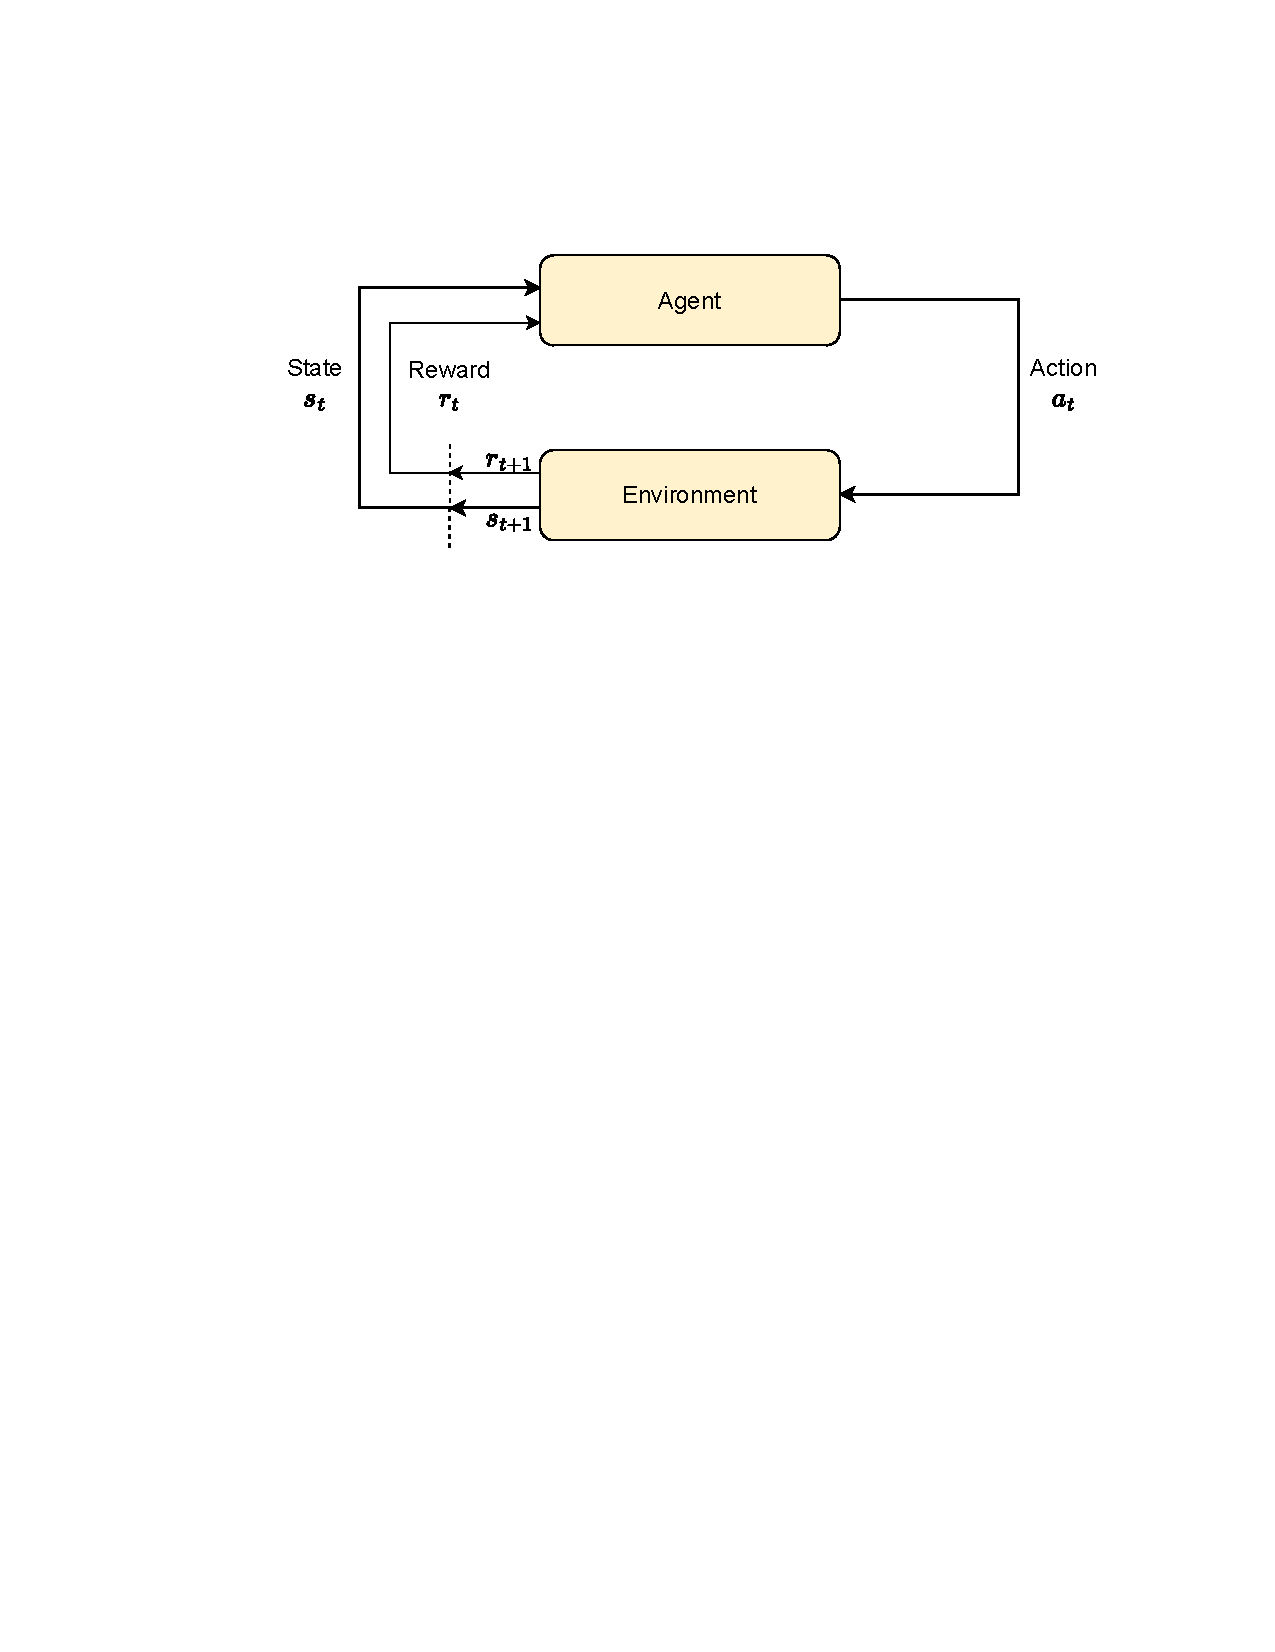
\includegraphics[clip, trim=3cm 18cm 3cm 3cm, width=1.0\textwidth]{figures/rl}
	\caption{The figure shows the general reinforcement learning setting, where an agent interacts with an environment. The agent applies an action on the environment at each time step 
	and receives the next state and a reward. The figure was taken from Sutton et al.~\cite{Sutton1998RL}.}
	\label{fig:rl}
\end{figure}

where $\Psi_t$ is a value estimating the returns or advantages as described below, and the expectation is again 
taken over episodes sampled from the current policy $\pi_\theta(a_t | s_t)$. As usual, the gradient 
steps are done in batches of episodes via gradient descent, as shown in Section~\ref{sec:approach-description}. 

The value $\Psi_t$ can take several forms~\cite{Schulman2016GAE}. In the following, we 
introduce three of them, the Monte-Carlo return, the advantage, and GAE~\cite{Schulman2016GAE}.

\paragraph{Monte-Carlo Return}

The first option is the Monte-Carlo return~\cite{Schulman2016GAE, Peng2018Mimic}, also called the reward to go. The Monte-Carlo return computes the sum of rewards from 
step $t$ onwards and is defined as: 
\begin{equation}
	R_t = \sum_{i=0}^{T-t} \gamma^{i} \, r_{t+i}
	\label{eq:return}
\end{equation}
where $r_t$ are the rewards from the environment at each time step $t$ and $\gamma$ is the discount factor.
Setting $\Psi_t = R_t$ yields the REINFORCE~\cite{Williams1992REINFORCE} algorithm.
In this setup, $R_t$ determines the direction of the gradient update in Equation~\ref{eq:polupdate}. It should increase the probability 
of actions $a_t$ that lead to positive rewards and decrease the probability of actions leading to negative rewards.

However, while the Monte-Carlo return is an unbiased estimate of the expected return, it has a very high variance because each reward $r_t$ is a random variable that depends on randomness 
coming from the policy network $\pi_{\theta}(a_t | s_t)$~\cite{Peng2018Mimic}.\footnote{In case of probabilistic transition functions, there is also additional randomness coming from the environment.}
One possibility to reduce the variance while keeping the estimate unbiased is the substraction of a baseline $b_t$, such that $\Psi_t = R_t - b_t$~\cite{Mnih2016A2C}.
For example, $b_t$ could be a moving average of the Monte-Carlo return~\cite{Das2018Minerva}.


\paragraph{Advantage}
Another option to decrease the variance of the estimate is the introduction of a critic~\cite{Sutton1998RL}. In the resulting 
Actor-Critic setting, we have our policy network $\pi_\theta(a_t | s_t)$ representing the actor and a value network $V_\psi(s_t)$ parametrized by $\psi$ representing the critic.
The value network $V_\psi(s_t)$ should predict the value of the state $s_t$. In the 
Synchronous Advantage Actor-Critic (A2C) algorithm~\cite{Mnih2016A2C}, the value network is trained to predict the 
Monte-Carlo return $R_t$ from Equation~\ref{eq:return}. Subsequently, the advantage is defined as:
\begin{equation}
	\mathcal{A}_t^\psi = R_t - V_\psi(s_t)
	\label{eq:advantage}
\end{equation}
A2C then sets $\Psi_t = \mathcal{A}_t^\psi$ and uses Equation~\ref{eq:polupdate} to update the policy network.
In this case, the advantage $\mathcal{A}_t$ determines the direction of the gradient update. It increases or decreases the 
probability of actions $a_t$ depending on whether they are better or worse than average~\cite{Schulman2016GAE}.
Simultaneously, the value network is updated via the mean-squared error between the predictions 
of the value network $V_\psi(s_t)$ and the Monte-Carlo return $R_t$.

\paragraph{Generalized Advantage Estimation (GAE)}
Alternatively, we can replace the advantage in the policy network update with the 
generalized advantage estimate (GAE)~\cite{Schulman2016GAE} to further reduce the variance and achieve more control over the trade-off between bias and variance. Similarly, we can replace the Monte-Carlo return in the value network 
update with the $\lambda$-return~\cite{Sutton1998RL}.
In the following, we introduce the GAE and $\lambda$-return following the 
explanation from Peng et al.~\cite{Peng2018Mimic}.

Until now, the expected return is estimated via the unbiased Monte-Carlo 
return (Equation~\ref{eq:return}).
As discussed above, this estimator has a very high variance.
To address this problem, we can introduce $n$-step returns to decrease the variance.
The $n$-step return does not compute the complete sum until time step $T$ like the Monte-Carlo
return. Instead, the sum is computed for $n$ steps, and after that point, the estimate is 
bootstrapped via the value network $V_\psi(s_{t+n})$~\cite{Silver2015RL, Peng2018Mimic}:
\begin{equation}
	R_t^{(n)} = \sum_{i=0}^{n-1} \gamma^i \, r_{t+i} + \gamma^n V_{\psi} (s_{t+n}) 
\end{equation}
The disadvantage is that the bootstrap estimate via the value network introduces some bias.
Hence, the parameter $n$ can be used to control the trade-off between 
bias and variance. Specifically, high $n$ yield a lower bias but higher variance, whereas 
small $n$ yield a higher bias but lower variance. For example, setting $n=\infty$ gives us the 
Monte-Carlo return $R_t$ from Equation~\ref{eq:return}, assuming that all rewards after the maximum 
episode length $T$ are $0$~\cite{Peng2018Mimic}.

However, now arises the question of which $n$ we should choose. We could treat it as 
a hyperparameter and optimize the setting on some validation set.
Instead, the literature introduced the $\lambda$-return~\cite{Sutton1998RL} to deal with this problem.
The $\lambda$-return does not take a specific $n$ but rather computes the exponentially 
weighted average over all of them~\cite{Peng2018Mimic}: 
\begin{equation}
	%\vspace{-1cm}
	R_t(\lambda) \stackrel{(1)}{=} (1- \lambda) \sum_{n=1}^{\infty} \lambda^{n-1} R_t^{(n)} \stackrel{(2)}{=} (1-\lambda) \sum_{n=1}^{T-t-1} \lambda^{n-1} \, R_t^{(n)} + \lambda^{T-t-1} R_t^{(T-t)} 
\end{equation}
where $\lambda$ is a hyperparameter between $0$ and $1$, which can be used to control the trade-off between bias and variance. Equality (1) shows the general
form of the $\lambda$-return up to infinity. Equality (2) holds if all  
rewards after time step $T$ are $0$~\cite{Peng2018Mimic}. For more details, see 
the appendix of Peng et al.~\cite{Peng2018Mimic}.

Finally, we set the advantage in Equation~\ref{eq:advantage} to $\mathcal{A}_t^{\psi} = R_t(\lambda) - V_\psi(s_t)$, 
which corresponds to the GAE~\cite{Schulman2016GAE}.
Moreover, we optimize the value network via the mean-squared error between the predictions of the value network $V_\psi(s_t)$ and the
$\lambda$-returns $R_t(\lambda)$~\cite{Peng2018Mimic}, as shown in Section~\ref{sec:approach-description}.

%\section{Language Models}
%\label{subsec:language-models}


%\paragraph{Notation}

%\begin{itemize}
	%\item entities in the graph $e \in \mathcal{E}$
	%\item question $q$
	%\item question embedding $q_{emb}$
	%\item cause and effect from question $e_c$ and $e_e$
	%\item state $s_t = (q, e_t, h_t)$ or $(q_{emb}, e_{t_{emb}}, h_t)$
	%\item action $a_t = e_{t+1}$
	%\item path rollout $p=((s_0,a_0),(s_1, a_1), \dots, (a_{T_1}, s_{T-1}))$
	%\item mathbf for embeddings
	%\item maybe converter function?
%\end{itemize}






         % INCLUDE: approach
% !TEX root = my-thesis.tex

\chapter{Approach}
\label{ch:approach}
In the following, we describe our approach in detail. First, we provide the concrete problem definition. Second,
we introduce the environment details and formulate the question-answering task as a sequential decision problem on a causal knowledge graph.
Afterward, we present our reinforcement learning agent for
causal question answering. This includes the network architecture, the training 
procedure, and the search strategy at inference time.
Finally, we discuss extensions like bootstrapping with supervised learning and
reward-shaping techniques.

%\section{Dataset Curation}
%\label{sec:dataset-curation}

\section{Problem Definition}
\label{sec:problem-def-env}

Given a causal question $q$ in natural language and a causal knowledge graph $\mathcal{K} = (\mathcal{E}, \mathcal{R})$,
the reinforcement learning agent 
walks over the graph to answer the question. 
Note that, the given causal knowledge graph only contains the \textit{cause} relation such that 
$\mathcal{R} = \{cause\}$.
In particular, the search should be as efficient as 
possible. In the ideal case, it should run in under half a second to give users an answer
in a reasonable time frame~\cite{Arapakis2014Search}.
We consider binary causal questions $q$, where the agent must determine the validity
 of a causal relation. The curation of our binary causal question dataset was described 
 in detail in Section~\ref{subsec:causal-questions}. To reiterate, we consider 
 binary causal questions like \textit{``Can X cause Y?''} which contain exactly one 
 cause and one effect.

In the following, we elucidate the binary causal question answering task on the knowledge graph 
$\mathcal{K}$ on the basis of the example in Figure~\ref{fig:graph_example}.
The example shows an excerpt of a causal knowledge graph (CauseNet) and the 
binary causal question \textit{``Does pneumonia cause anemia?''}. In this question, 
\textit{pneumonia} takes the role of the cause, and \textit{anemia} the role of the effect.

First, the cause and effect are linked to the graph. Specifically, we find entities $e_c, e_e \in \mathcal{E}$
such that \textit{pneumonia} maps to $e_c$ and \textit{anemia} to $e_e$. Currently, we 
link them via exact string matching. However, 
more sophisticated strategies can be considered in future work~\cite{Kaiser2021Reinforcement}.
Consequently, starting from $e_c$
the agent has to find a path $(e_c, e_1, e_2, \dots, e_e)$ with $e_i \in \mathcal{E}$, where the agent arrives at the effect $e_e$.\footnote{The relations on the path were omitted, because the graph contains only one relation type.} 
If the agent finds such a path, the question is answered with ``yes'' and with ``no'' otherwise.
For the example, a possible path is \textit{(pneumonia, sepsis, kidney  failure, anemia)}.
Afterward, we can
inspect the path to get further insights into the relationship between cause and effect.

\begin{table}[t]
\caption{Eight cause-effect pairs randomly sampled from CauseNet. The table shows the number of paths of length two starting at the cause (\textit{|Paths|}) compared to
		 the number of paths between the cause and effect (\textit{|Solutions|}), \textbf{not including} inverse edges.
		}
\label{table-path-complexity}
\centering
\begin{tabular}{llrr} 
			\toprule
			\textbf{Cause} & \textbf{Effect} & \textbf{|Paths|} & \textbf{|Solutions|}\\
			\midrule
		   accident & death & 18,967 & 173 \\
		   heart failure & angina &	3,533 &	5	\\
		   pneumonia & dehydration &	7,662 &	18	\\
		   cancer & abnormalities &	24,168 &	20	\\
		   illness & suicidal behavior & 25,226 &	3	\\
		   stroke  & pain	& 10,700 & 55 \\
		   complications & confusion & 12,839 &	19	\\
		   infection & abdominal pain &28,955 &	53	\\
			\bottomrule
\end{tabular}
\bigskip
\caption{Eight cause-effect pairs randomly sampled from CauseNet. The table shows the number of paths of length two starting at the cause (\textit{|Paths|}) compared to
		 the number of paths between the cause and effect (\textit{|Solutions|}), \textbf{including} inverse edges.
}
\label{table-path-complexity-inverse}
\centering
\begin{tabular}{llrr} 
			\toprule
			\textbf{Cause} & \textbf{Effect} & \textbf{|Paths|} & \textbf{|Solutions|} \\
			\midrule
		   accident & death & 117,952 & 466 \\
		   heart failure & angina &	71,892 &	27	\\
		   pneumonia & dehydration &	66,715 &	84	\\
		   cancer & abnormalities &	160,000 &	82	\\
		   illness & suicidal behavior & 192,224 &	13	\\
		   stroke  & pain	& 109,305 & 255 \\
		   complications & confusion & 152,593 & 138 \\
		   infection & abdominal pain & 163,487 &	97	\\
			\bottomrule
\end{tabular}
\end{table}

\paragraph{Challenges}
Contrary to previous approaches for reinforcement learning on 
knowledge graphs~\cite{Xiong2017DeePpath, Das2018Minerva, Qiu2020Stepwise}, our causal 
knowledge graph only contains one 
 relation type, i.e., $\mathcal{R} = \{cause\}$.
Thus, the relations do not provide any learning signal, which makes the question
 answering task particularly challenging.
Prior approaches, such as \textit{DeepPath}~\cite{Xiong2017DeePpath} or \textit{MINERVA}~\cite{Das2018Minerva},
used knowledge graphs with multiple relation types. This enabled them to use the 
relations types as actions at each time step. In our case, the action space consists 
of all entities $\mathcal{E}$ in the graph. 
%Even more important, the action the agent can
%take change at each time step, due to the different neighborhoods of each entity.

For example, we use CauseNet~\cite{Heindorf2020Causenet} to illustrate these challenges in more detail.
CauseNet-Precision contains 80,223 entities (Table~\ref{table-causenet}), where 
each entity corresponds to an action for our agent. In comparison, prior works considered
graphs with only up to 237 relation types~\cite{Das2018Minerva} which they used as actions.
Table~\ref{table-path-complexity} shows eight cause-effect pairs 
sampled from CauseNet. The \textit{|Paths|} column shows the total number of paths 
of length two starting from the \textit{cause}, while the \textit{|Solution|} column 
shows the number of paths of length two between the \textit{cause} and \textit{effect}.
Table~\ref{table-path-complexity-inverse} shows the same statistics with inverse edges 
included. These numbers further demonstrate the huge action space, with some examples having over 100,000 paths of length two, where each unique entity on these paths corresponds to a 
different action. 


%While the average degree of CauseNet is only x, there are 

To address these challenges, we experiment with different techniques to improve the 
reinforcement learning agent. For example, via supervised learning to bootstrap the agent
 at the beginning of learning~\cite{Xiong2017DeePpath}, which we discuss in Section~\ref{sec:supervised}. This way,
 the agent receives correct paths at the start to help navigate the large action space.

%%\begin{table}
%\caption{The left column shows a list of patterns for binary causal question. To illustrate, \texttt{cause}
%		 and \texttt{effect} can be arbitrary phrases, while \texttt{\pattern{cue\_word}} is a 
%		 causal cue word from the right column. The right column shows a selection of causal cue words
%		 with low ambiguity and high frequency~\cite{Girju2002CausalCue}. For the full lists
%		 of causal patterns and cue words see the Appendix.}
%\label{table-patterns}
%\centering
%\begin{tabular}{ll}
%	\toprule
%	\textbf{ID} & \textbf{Causal Question Patterns}\\
%	\toprule
%	\textbf{P1:} & {\small can} \pattern{cause} \pattern{cue\_word} \pattern{effect} \\
%	\textbf{P2:} & {\small is} \pattern{effect} \pattern{cue\_word} {\small by} \pattern{cause} \\
%	\textbf{P3:} & {\small could} \pattern{cause} \pattern{cue\_word} \pattern{effect}\\
%	\textbf{P4:} & {\small might} \pattern{cause} \pattern{cue\_word} \pattern{effect}\\
%	\textbf{P5:} & {\small would} \pattern{cause} \pattern{cue\_word} \pattern{effect}\\
%	\textbf{P6:} & \pattern{cause} \pattern{cue\_word} \pattern{effect}\\
%	\bottomrule
%	\end{tabular}
%	\quad
%	\begin{tabular}{r}
%	\toprule
%	\textbf{Causal Cue Words}\\
%	\toprule
%	cause \\
%	induce \\
%	produce \\
%	effect \\
%	lead (to) \\
%	result \\
%	\bottomrule
%	\end{tabular}
%\end{table}
\begin{table}
\caption{Number of paths of length two starting at the cause (\textit{Paths}) compared to
		 the number of paths between the cause and effect (\textit{Solutions}). Without 
		 inverse edges.}
\label{table-path-complexity}
\centering
\begin{tabular}{llrr} 
			\toprule
			\textbf{Cause} & \textbf{Effect} & \textbf{|Paths|} & \textbf{|Solutions|}\\
			\toprule
		   accident & death & 18.967 & 173 \\
		   heart failure & angina &	3.533 &	5	\\
		   pneumonia & dehydration &	7.662 &	18	\\
		   cancer & abnormalities &	24.168 &	20	\\
		   heart attack & death of & 7.395 &	1	\\
		   illness & suicidal behavior & 25.226 &	3	\\
		   stroke  & pain	& 10,700 & 55 \\
		   complications & confusion & 12.839 &	19	\\
		   infection & abdominal pain &28.955 &	53	\\
			\bottomrule
\end{tabular}
\end{table}
\begin{table}
\caption{Number of paths of length two starting at the cause (\textit{Paths}) compared to
		 the number of paths between the cause and effect (\textit{Solutions}). Including 
		 inverse edges.}
\label{table-path-complexity-inverse}
\centering
\begin{tabular}{llrr} 
			\toprule
			\textbf{Cause} & \textbf{Effect} & \textbf{|Paths|} & \textbf{|Solutions|} \\
			\toprule
		   accident & death & 117.952 & 466 \\
		   heart failure & angina &	71.892 &	27	\\
		   pneumonia & dehydration &	66.715 &	84	\\
		   cancer & abnormalities &	160.000 &	82	\\
		   heart attack & death of & 96.144 &	1	\\
		   illness & suicidal behavior & 192.224 &	13	\\
		   stroke  & pain	& 109.305 & 255 \\
		   complications & confusion & 152.593 & 138 \\
		   infection & abdominal pain & 163.487 &	97	\\
			\bottomrule
\end{tabular}
\end{table}


\section{Environment}
\label{sec:env}
As done by related work~\cite{Xiong2017DeePpath, Das2018Minerva, Qiu2020Stepwise}, we formulate the causal question answering task as a sequential decision
problem on the knowledge graph $\mathcal{K}$. The agent walks over the graph and decides which
relation to take at each entity. Therefore, we define a Markov Decision Process (MDP) as a 4-tuple 
$(\mathcal{S}, \mathcal{A}, \delta, \mathcal{R})$. The MDP consists of the state space $\mathcal{S}$,
 the action space $\mathcal{A}$, the transition function $\delta : \mathcal{S} \times 
 \mathcal{A} \rightarrow \mathcal{S}$, and the reward function 
 $\mathcal{R} : \mathcal{S} \rightarrow \mathbb{R}$. Hence, at each state $s_t \in \mathcal{S}$ the agent selects
 an action $a_t \in \mathcal{A}$, which changes the current state via $\delta(s_t, a_t)$ to 
 $s_{t+1}$. Additionally, the agent receives a reward $\mathcal{R}(s_{t+1}) = r_t$.
 Note that the transition function $\delta$ is known and deterministic because the graph entirely defines $\delta$.
 So, for each action $a_t$ in state $s_t$, the
 next state $s_{t+1}$ is known.

 \paragraph{Agent} Our agent consists of a policy network $\pi_{\theta} (a_t | s_t)$ (Actor)
 parametrized with $\theta$ and a value network $V_{\psi}(s_t)$ (Critic) parametrized with $\psi$. The policy network $\pi_{\theta} (a_t | s_t)$ generates
 a distribution over actions $a_t$ at the current state $s_t$. The value network
$V_{\psi}(s_t)$ generates a scalar to estimate the value of the state $s_t$.
More specifically, the value network should predict the future reward from state $s_t$ onwards.

\paragraph{States} At each time step t, we define the state $s_t = (\mathbf{q}, e_t, \mathbf{e_t}, \mathbf{h_t}, e_e) \in \mathcal{S}$,
where $\mathbf{q}$ represents the embedding of the question $q$, $e_t \in \mathcal{E}$ the current entity, and $\mathbf{e_t}$ its embedding. 
The entity $e_t$ is needed to define the action space, and its embedding $\mathbf{e_t}$ is used as input to the agent's networks.
Additionally, $\mathbf{h_t}$ represents the path history of the agent and $e_e$ the entity corresponding to the effect found in the question $q$.
Moreover, $e_0 = e_c$ and $\mathbf{h_0} = \mathbf{0}$, where $e_c$ is the entity 
corresponding to the cause of the question (e.g., \textit{pneumonia} in the example in 
Figure~\ref{fig:graph_example}). The path history is represented by the hidden states of an
LSTM. 

\paragraph{Actions} The action space at each time step $t$ consists of all neighboring
entities of the current entity in state $s_t$. Therefore, the set of possible actions in 
state $s_t = (\mathbf{q}, e_t, \mathbf{e_t}, \mathbf{h_t}, e_e)$ is defined as $A(s_t) = \{e | (e_t, r, e) \in \mathcal{K}\}$ where $r = cause$.
So only the current entity $e_t$ is needed to define the
action space $A(s_t)$. Note that while the additional components inside the state
are not needed to define the action space, they are needed for other parts 
of the learning algorithm, as described below in 
 Sections~\ref{sec:approach-description} and~\ref{sec:network}. 

 As described in Section~\ref{subsec:causal-kgs}, CauseNet~\cite{Heindorf2020Causenet} contains
 additional meta-information for each relation in the form of the original sentence $s$.
 Therefore, we include the original sentence $s$ when computing the embedding $\mathbf{a_t}$ for an action $a_t$.
 This is done by concatenating the sentence embedding $\mathbf{s}$ with the embedding of the chosen
 entity $e = a_t$. Thus, the action embedding becomes $\mathbf{a_t} = [\mathbf{s};\mathbf{e}]$.

As done by prior works~\cite{Das2018Minerva, Lin2020RewardShaping, Qiu2020Stepwise}, we add a special \textit{STAY} action at each step, so the action space becomes $A(s_t) = A(s_t) \cup \{STAY\}$. 
When selecting this action, the agent stays at the current entity. This way, we can keep 
all episodes to the same length, even though different questions might require a different
 number of hops. Another option would be to add a stop action. However, in that case,
 we would have episodes of different lengths.\footnote{In principle, episodes of different lengths are not a problem. However, keeping them to the same length simplifies the implementation. We chose this simplification because it worked well in prior works~\cite{Das2018Minerva, Qiu2020Stepwise}.}
 Moreover, we add inverse edges to the graph because our experiments showed that 
 their addition increases the performance. In general, inverse edges allow the agent to undo wrong decisions and to reach nodes 
 that could otherwise not be reached under a given episode length. We discuss some implications and tradeoffs regarding 
 inverse edges in Chapter~\ref{ch:discussion}.

\paragraph{Transitions}
As described above, the transition function is deterministic, meaning the next 
state is fixed after the agent 
selects an action. Let $s_t=(\mathbf{q}, e_t, \mathbf{e_t}, \mathbf{h_t}, e_e)$ be the 
current state and $a_t \in A(s_t)$ be the action the agent selected in state $s_t$.
Subsequently, the environment evolves via $\delta(s_t, a_t)$ to $s_{t+1}=(\mathbf{q}, e_{t+1}, \mathbf{e_{t+1}}, \mathbf{h_{t+1}}, e_e)$,
where $e_{t+1}=a_t$.  

\paragraph{Rewards}
In the default setup, the agent only receives a terminal reward at the final time step $T-1$. 
Specifically, the agent receives a reward of $\mathcal{R}(s_{T-1}) = 1$ if $s_{T-1} = (\mathbf{q}, e_{T-1}, \mathbf{e_{T-1}}, \mathbf{h_{T-1}}, e_e)$ with 
$e_{T-1} = e_e$. Conversely,
the agent receives a reward of $\mathcal{R}(s_{T-1}) =0$ if $e_{T-1} \neq e_e$. Similarly, for all other 
time steps, with $t < T -1$, the reward is $0$ as well. This setup inhibits the typical
sparse reward problem found in many reinforcement learning applications. Thus, we
experimented with reward-shaping techniques similar to related work~\cite{Lin2020RewardShaping,Yasunaga2021QAGNN}.
For more details, see Section~\ref{sec:reward-shaping}.

\paragraph{Path Rollouts --- Episodes}
We define a path rollout or episode as a sequence of three tuples containing 
a state, action, and reward. Assuming a path rollout length of $T$, an example
for a path rollout is: $((s_0, a_0, r_0),\dots, (s_{T-2}, a_{T-2}, r_{T-2}))$.
For path rollout length $T$, a path rollout contains $T-1$ tuples.
This is because the last state $s_{T-1}$ is only needed for the calculation of reward
$r_{T-2}$, and no further action is taken.\footnote{See Algorithm~\ref{alg:algorithm} Lines \ref{ln:17}-22 for more details.}
For brevity, the rewards $r_t$ can be omitted.


\begin{figure}
    \centering
    \small
    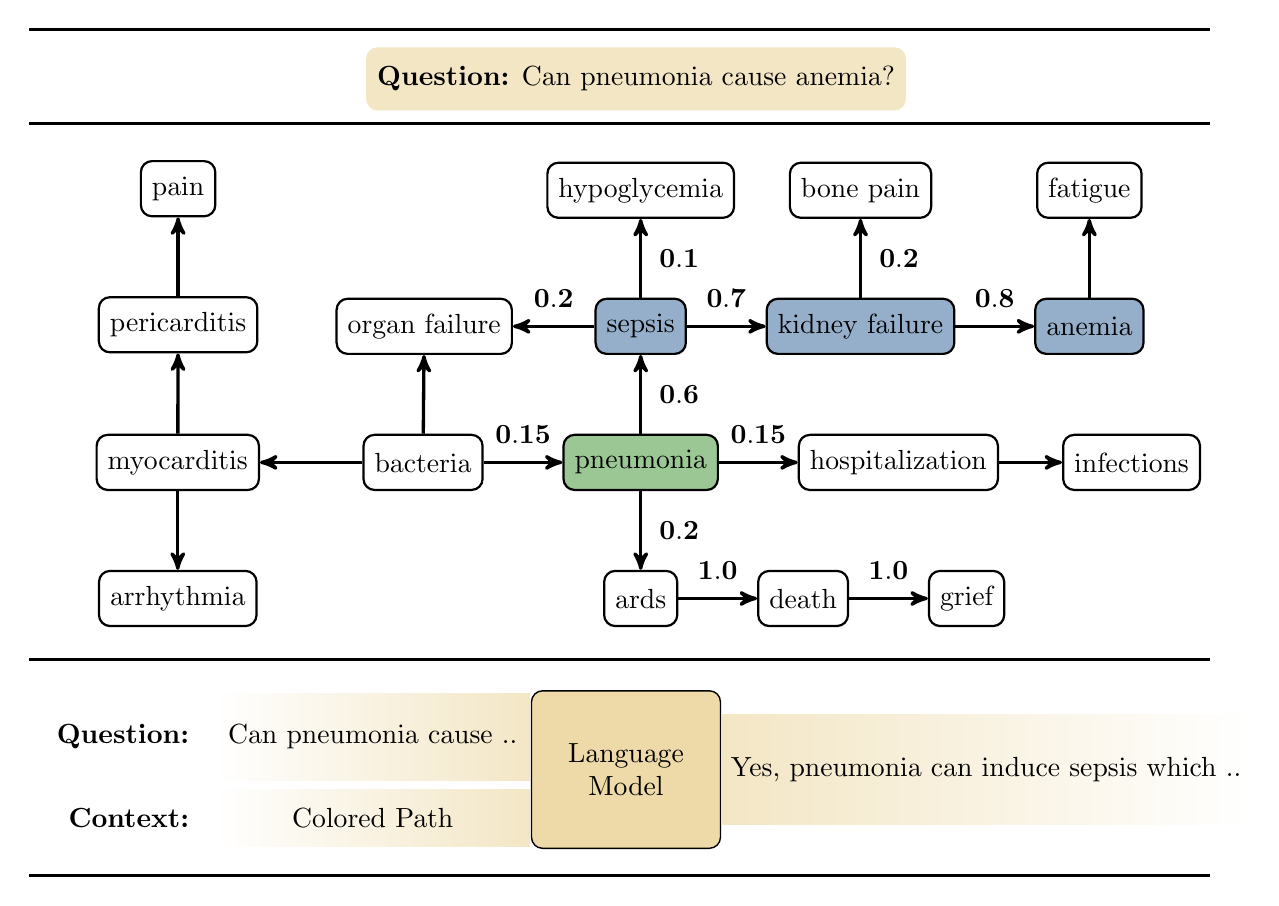
\begin{tikzpicture}
        %\tikzstyle{vertex}=[draw, rectangle, rounded corners, minimum width=1.8cm, minimum height=1.4cm, line width=0.8pt]
        \tikzstyle{vertex}=[draw, rounded corners, line width=0.8pt, inner sep=4pt, minimum height = 0.7cm]
        \tikzstyle{box}=[minimum height=0.8cm, minimum width = 6cm, inner sep=4pt, rounded corners]
        \tikzstyle{arrow} = [->, thick,>=stealth']
        
        
        %\node[draw, line width=1pt] (Corner) {};
        \node[vertex] (N1) {bacteria};
        \node[vertex, left = 1.3cm of N1] (myocarditis) {myocarditis};
        \node[vertex, below = 1cm of myocarditis] (arrhythmia) {arrhythmia};
        \node[vertex, above left = 1.02cm and 1.32cm of N1] (pericarditis) {pericarditis};
        \node[vertex, above = 1cm of pericarditis] (pain) {pain};
        \node[vertex, right = 1cm of N1, fill=tab20darkgreen!60] (pneumonia) {pneumonia};
        \node[vertex, right = 1cm of pneumonia] (hospitalization) {hospitalization};
        \node[vertex, right = 0.8cm of hospitalization] (infections) {infections};
        \node[vertex, above = 1cm  of pneumonia, fill=tab20darkblue!60] (sepsis) {sepsis};
        \node[vertex, above = 1cm of sepsis] (hypoglycemia) {hypoglycemia};
        \node[vertex, left = 1.035cm of sepsis] (organ) {organ failure};
        \node[vertex, below = 1cm of pneumonia] (ards) {ards};
        \node[vertex, right = 1cm of ards] (death) {death};
        \node[vertex, right = 1cm of death] (grief) {grief};
        
        \node[vertex, right = 1cm  of sepsis, fill=tab20darkblue!60] (kidney) {kidney failure};
        \node[vertex, above = 1cm  of kidney] (bone) {bone pain};
        \node[vertex, right = 1cm  of kidney, fill=tab20darkblue!60] (anemia) {anemia};
        \node[vertex, above = 1cm  of anemia] (fatigue) {fatigue};
        
         \node[draw, rounded corners, line width=0.5pt, inner sep=4pt,below left = 0.8cm and -1.5cm of ards, fill=brass!60, minimum height=2cm, minimum width = 2.4cm, align=center] (LM) {Language \\ Model};
         
        \node[box, fill=brass!40, label=left:{}, above right = 4.1cm and -1.5cm of N1] (MCQ)  {\textbf{Question:} Can pneumonia cause anemia?};
         
         \node[left color=white, right color=brass!40, above left = -1.15cm and 0cm of LM, fill=brass!40, minimum height=1.1cm, minimum width = 4cm, align=center] (q1) {Can pneumonia cause ..};
         \node[left color=white, right color=brass!40, below = 0.1cm of q1, fill=brass!40, minimum height=0.73cm, minimum width = 4cm, align=center] (q2) {Colored Path};
         \node[left = 0.2cm of q1, fill=white, minimum height=1.1cm, minimum width = 1.5cm, align=center] (t1) {\textbf{Question:}};
         \node[left = 0.2cm of q2, fill=white, minimum height=1.1cm, minimum width = 1.5cm, align=center] (t2) {\textbf{Context:}};
         \node[right color=white, left color=brass!40, right = 0cm of LM, fill=brass!40, minimum height=1.4cm, minimum width = 4cm, align=center] (q3) {Yes, pneumonia can induce sepsis which ..};

        
        %\node[above left = 0.3cm and -0.4cm of pericarditis] (a) {\textbf{a)}};
        %\node[above left = 0.2cm and -0.5cm of MCQ] (b) {\textbf{b)}};
        %\node[below left = 0.35cm and 3.4cm of ards] (c) {\textbf{c)}};

        %\node[left = 0.1cm of sepsis] (ps) {\textbf{0.7}};
        %\node[above = 0.1cm of pneumonia] (pf) {\textbf{0.1}};
        %\node[left = 0.1cm of ards] (pa) {\textbf{0.2}};
        %\node[above = 0.1cm of death] (pa) {\textbf{1.0}};
        %\node[above = 0.1cm of kidney] (ph) {\textbf{1.0}};
        
        \draw[arrow, line width=1.2pt] (N1) -- (myocarditis);
        \draw[arrow, line width=1.2pt] (N1) -- (organ);
        \draw[arrow, line width=1.2pt] (pneumonia) to node[right=0.1cm, pos=0.5]  {$\mathbf{0.6}$} (sepsis);
        \draw[arrow, line width=1.2pt] (pneumonia)  to node[right=0.1cm, pos=0.5]  {$\mathbf{0.2}$}(ards);
        \draw[arrow, line width=1.2pt] (pneumonia) to node[above=0.1cm, pos=0.5]  {$\mathbf{0.15}$} (hospitalization);
        \draw[arrow, line width=1.2pt] (N1) to node[above=0.1cm, pos=0.5]  {$\mathbf{0.15}$} (pneumonia);
        \draw[arrow, line width=1.2pt] (kidney) to node[above=0.1cm, pos=0.5]  {$\mathbf{0.8}$} (anemia);
        \draw[arrow, line width=1.2pt] (kidney) to node[right=0.1cm, pos=0.5]  {$\mathbf{0.2}$} (bone);
        \draw[arrow, line width=1.2pt] (anemia) -- (fatigue);
        \draw[arrow, line width=1.2pt] (hospitalization) -- (infections);
        \draw[arrow, line width=1.2pt] (sepsis) to node[right=0.1cm, pos=0.5]  {$\mathbf{0.1}$} (hypoglycemia);
        \draw[arrow, line width=1.2pt] (sepsis) to node[above=0.1cm, pos=0.5]  {$\mathbf{0.2}$} (organ);
        \draw[arrow, line width=1.2pt] (myocarditis) -- (pericarditis);
        \draw[arrow, line width=1.2pt] (myocarditis) -- (arrhythmia);
        \draw[arrow, line width=1.2pt] (pericarditis) -- (pain);
        
        \draw[arrow, line width=1.2pt] (sepsis) to node[above=0.1cm, pos=0.5]  {$\mathbf{0.7}$} (kidney);
        \draw[arrow, line width=1.2pt] (ards) to  node[above=0.1cm, pos=0.5]  {$\mathbf{1.0}$} (death);
        \draw[arrow, line width=1.2pt] (death) to  node[above=0.1cm, pos=0.5]  {$\mathbf{1.0}$} (grief);

        \draw [draw, line width=1.2pt] (-5,5.5) -- (10,5.5);
        \draw [draw, line width=1.2pt] (-5,4.3) -- (10,4.3);
        \draw [draw, line width=1.2pt] (-5,-2.5) -- (10,-2.5);
        \draw [draw, line width=1.2pt] (-5,-5.25) -- (10,-5.25);
        %\draw[thick,rounded corners]     ($(inflammation.north west)+(-0.2,0.89)$) rectangle ($(death.south east)+(0.5,-0.3)$);
        
        %\draw[thick,rounded corners]     ($(ards.south west)+(-4,-0.3)$) rectangle ($(C.south east)+(0.5,-3)$);
    \end{tikzpicture}
    \caption{An excerpt from CauseNet~\cite{Heindorf2020Causenet} showing the entity \textit{pneumonia} together with its neighborhood containing causes and effects. 
            Each edge depicts a \textit{cause} relation. Given the question \textit{``Can pneumonia cause anemia?''}, the search
            starts at the entity \textit{pneumonia}. Following the path \textit{(pneumonia, sepsis, kidney failure, anemia)}, the question 
            can be answered with ``yes''. The numbers on the edges show the probability of taking this edge under the current 
            policy $\pi_{\theta}(a_t | s_t)$. For brevity, we only show the relevant probabilities for the given path. The lower part of the figure shows the possibility to combine our agent with a language model. In that setup, we provide the paths the agent learned for a question as additional context 
            to the language model. We briefly explore this setup in Section~\ref{sec:evaluation-approach}.
            }
    \label{fig:graph_example}
\end{figure}

\section{Network Architecture}
\label{sec:network}
 We use a Long Short-Term Memory (LSTM)~\cite{Hochreiter1997LSTM} to parametrize our agent. LSTMs were introduced to improve 
 standard RNNs and can better handle the vanishing gradient problem~\cite{Hochreiter1997LSTM}. 
 Additionally, we experimented with a simple feedforward architecture 
 but found that incorporating the path history is crucial for our needs.
 This aligns with previous research, where approaches such as MINERVA~\cite{Das2018Minerva} and SRN~\cite{Qiu2020Stepwise} 
 also used LSTMs and GRUs. Just CONQUER~\cite{Kaiser2021Reinforcement} used a feedforward architecture, but they only 
 considered paths of length one.


 Let $\mathbf{q} \in \mathcal{R}^d$ be the embedding of the question $q$ and $\mathbf{E} \in \mathcal{R}^{|\mathcal{E}| \times d}$ the 
 embedding matrix containing the embeddings for each entity $e \in \mathcal{E}$ of the knowledge graph.
 The parameter $d$ specifies the dimension of the embeddings.
  $\mathcal{K}$. The LSTM formula is then applied as follows:

\begin{equation}
	\mathbf{h_t}=
    \begin{cases}
      LSTM(\mathbf{0}; [\mathbf{q}, \mathbf{e_c}]), & \text{if}\ t=0 \\
      LSTM(\mathbf{h_{t-1}}, [\mathbf{q}; \mathbf{e_t}]), & \text{otherwise}
    \end{cases}
\end{equation}

where $\mathbf{h_t} \in \mathcal{R}^{2d}$ represents the hidden state vector (history) of the LSTM, 
and $[;]$ is the vector concatenation operator. At each time step, the LSTM takes the previous history
 $\mathbf{h_{t-1}}$ and the concatenation of the question embedding $\mathbf{q}$ and the current node embedding
 $\mathbf{e_t} \in \mathcal{R}^{d}$ to produce $\mathbf{h_t}$. In the first time step, $\mathbf{h_0}$ is initialized with the
 zero vector and $\mathbf{e_0} = \mathbf{e_c}$, where $\mathbf{e_c}$ is the embedding of the entity corresponding to 
 the cause found in the current question. 
 %Previous approaches like MINERVA~\cite{Das2018Minerva} also 
 %concatenated the previous action embedding $\mathbf{a_{t-1}}$ to $\mathbf{e_t}$. However, 
 %we found this not to be necessary. Generally, it should be implicitly included through the
 %history $\mathbf{h_t}$.

 On top of the LSTM, we stack two feedforward networks: one for the policy 
 network $\pi_\theta(a_t | s_t)$ and one for the value network $V_\psi(s_t)$.
 In Section ~\ref{sec:env}, we defined the action space $\mathcal{A}(s_t)$ at time step $t$ and state $s_t = (\mathbf{q}, e_t, \mathbf{e_t}, \mathbf{h_t}, e_e)$
  to contain all neighbors of the entity $e_t$.
  Therefore, we introduce an embedding matrix $\mathbf{A_t} \in \mathcal{R}^{|A(s_t)| \times 2d}$, where
  the rows contain the embeddings of the actions  $a_t \in \mathcal{A}(s_t)$. Consequently, 
  the output of the policy network $\pi_{\theta}(a_t|s_t)$ is computed as follows:
\begin{equation}
	\begin{split}
	\pi_\theta(a_t | s_t) = \sigma(\mathbf{A_t} \times W_2 \times ReLU(W_1 \times \mathbf{h_t})) \\
	a_t \sim Categorical(\pi_\theta(a_t | s_t))
	\end{split}
\end{equation}

where $W_1 \in \mathcal{R}^{h \times 2d}$ and $W_2 \in \mathcal{R}^{2d \times h}$ are weight matrices with hidden dimension $h$ and $\sigma$ is the softmax operator.
The final output of the policy network is a categorical probability distribution over 
all actions $a_t \in \mathcal{A}(s_t)$.
Similarly, the output of the value network $V_{\psi}(s_t)$ is computed with the 
following feedforward network:
\begin{equation}
	V_{\psi}(s_t) = W_4 \times ReLU(W_3 \times \mathbf{h_t})
\end{equation}
where $W_3\in \mathcal{R}^{h \times 2d}$ and $W_4\in \mathcal{R}^{1 \times h}$ are weight matrices with hidden dimension $h$, and the output is a scalar that
estimates the future reward from state $s_t$ onwards. Overall, the weights of
the LSTM are shared between the policy and value network, while each network 
has its own weights in the form of its feedforward head.


\section{Training of the Reinforcement Learning Agent}
\label{sec:approach-description}

In the following, we describe the training procedure of our reinforcement learning agent.
This includes the pre-processing of the questions, the sampling of path rollouts, and the update rules 
for the weights of the agent.
We start with the observation that CauseNet~\cite{Heindorf2020Causenet} does not contain 
negative information. Thus, we only train the agent on positive causal questions, i.e., questions 
whose answer is ``yes''. 
Similarly, we must remove all questions where the cause, effect, or both cannot be found in CauseNet. 
In that case, we are restricted by CauseNet, so there is nothing to learn.

%Training the agent on both, positive and negative questions, would result in 
%conflicting reward signals. For positive questions we would give the agent a reward of 
%one if a path is found and when given a negative question we would have to give a 
%reward of one when no path is found.

Algorithm~\ref{alg:algorithm} displays the pseudocode of the whole training phase.
The pseudocode assumes that only positive causal questions, where cause and effect can be found in 
CauseNet, remain in the given $questions$.
First, we pre-process the questions by linking the cause and effect to the corresponding 
entities $e_c$ and $e_e$ in CauseNet. This is followed by the computation of embeddings for the question and entities.\footnote{We use GloVe~\cite{Pennington2014Glove} embeddings to embed the questions and entities. For more details, see Section~\ref{sec:impl-details}}
Next, the weights $\theta$ and $\psi$ of the agent are initialized. 
In the default setup, both are initialized randomly.
In the case of a preceding supervised learning phase (Section~\ref{sec:supervised}), the weights 
of the policy network $\theta$ are initialized with the resulting weights from the supervised learning.

Afterward, we start sampling path rollouts from the environment via the current policy network
$\pi_\theta(a_t | s_t)$. Each path rollout has the same length $T$. Hence, the agent 
should learn to use the \textit{STAY} action in case it arrives at 
the target entity before a length of $T$ is reached. Given a pre-processed question $q$, we construct the first state $s_0$.
Subsequently, the agent interacts with the environment for $T$ time steps. At each time step, 
the agent applies an action $a_t$ and receives a reward $r_t$ while the environment evolves 
via the transition function $\delta(s_t, a_t)$ to the next state $s_{t+1}$.
This procedure is continued until a full batch of path rollouts is accumulated.


The training of the agent is facilitated via the Synchronous Advantage Actor-Critic (A2C)~\cite{Mnih2016A2C} algorithm, 
as described in Section~\ref{subsec:rl}. The policy network 
$\pi_\theta(a_t | s_t)$ takes the role of the actor while the value network $V_\theta(s_t)$ takes 
the role of the critic. We briefly experimented with Proximal Policy Optimization (PPO)~\cite{Schulman2017PPO} but found no significant performance improvements.

Thus, the update rule for the policy network $\pi_\theta(a_t | s_t)$ looks as follows:
\begin{equation}
  \nabla_{\theta} J(\theta) = - \frac{1}{B} \sum_{i}^{B} \sum_{t=0}^{T-2} \nabla_{\theta} \log(\pi_{\theta} (a_t | s_t)) \, \mathcal{A}_{t}^{\psi}
\end{equation}
where $B$ is the batch size, T the path rollout length, and $\mathcal{A}_{t}^{\psi}$
the generalized advantage estimate (GAE) as described in Section~\ref{subsec:rl}.

As commonly done, we add an entropy regularization term to the objective~\cite{Das2018Minerva, Kaiser2021Reinforcement}.
The entropy regularization should help the agent with the exploitation vs. exploration tradeoff.
Specifically, it should encourage exploration during training and stop the agent from getting 
stuck in local minima. Therefore, the resulting policy should be more robust and have a higher diversity
 of explored actions. We compute the average entropy of the action distribution of
 $\pi_{\theta}(a_t | s_t)$ over all actions $a_t \in \mathcal{A}(s_t)$ at each time step $t$ and take the average over the 
 whole batch:
\begin{equation}
	H_{\pi_\theta} = \frac{1}{B(T-1)} \sum_{i}^{B} \sum_{t=0}^{T-2} (- \hspace{-0.3cm}\sum_{a_t \in \mathcal{A}(s_t)} \pi_\theta(a_t | s_t)  \log \pi_\theta(a_t | s_t))
\end{equation}

The final update for the policy network becomes:
\begin{equation}
  \theta = \theta - lr \cdot(\nabla_{\theta} J(\theta) + \beta H_{\pi_\theta})
\end{equation}
where $lr$ is the learning rate and $\beta$ is a hyperparameter 
that determines the weight of the entropy regularization term.

Simultaneously, we update the value network $V_{\psi}(s_t)$ via the mean-squared error between 
the $\lambda$-return and the predictions of the value network:
\begin{equation}
		\nabla_{\psi} J(\psi)= \frac{1}{B (T-1)} \sum_{i}^{B} \sum_{t=0}^{T-2} \nabla_{\psi} (R_t(\lambda) - V_{\psi}(s_t))^2
\end{equation}
where $R_t(\lambda)$ is the $\lambda$-return as described in Section~\ref{subsec:rl}.
Therefore, the final update for the value network becomes:
\begin{equation}
  \psi = \psi - lr \cdot \nabla_{\psi} J(\psi)
\end{equation}
where $lr$ is the learning rate. In our experiments, we use the same learning rate
$lr$ for both networks. This is not compulsory and they could also use 
different learning rates. Overall, the training loop of selecting path rollouts and 
using them to update the policy and value networks is repeated for a number of 
optimization $steps$.

\begin{algorithm}
	\DontPrintSemicolon
	\caption{Pseudocode of the training procedure for the policy 
	network $\pi_{\theta}(a_t | s_t)$ and value network $V_\psi(s_t)$ 
	as described in Section~\ref{sec:approach-description}.}%
	\label{alg:algorithm}%
	\textbf{Input:} Knowledge graph $\mathcal{K}$, questions $questions$, 
	optimization steps $steps$, batch size $B$, path rollout length $T$, learning rate $lr$,
	entropy weight $\beta$, discount factor $\gamma$, GAE lambda $\lambda$  \\
	\textbf{Output:} Trained Agent $\theta$, $\psi$ \\
	\SetKwFunction{F}{TrainAgent}
	\SetKwProg{Fn}{Function}{:}{\KwRet $\theta$}
	\Fn{\F{$\mathcal{K}$, $questions$, $steps$, $B$, $T$, $lr$, $\beta$, $\gamma$, $\lambda$}}{%
		$processed\_questions = [ \ ]$\;
		\For{\textbf{each} $q$ \textbf{in} $questions$}{%
			Link the cause and effect of $q$ to entities $e_c$ and $e_e$ in $\mathcal{K}$\;
			Compute embeddings $\mathbf{q}$, $\mathbf{e_c}$ for $q$, $e_c$\;
			$processed\_questions.append((\mathbf{q}, e_c, \mathbf{e_c}, e_e))$
		}
		\;
		Initialize agent weights $\theta$, $\psi$\;
		$path\_rollouts = [\,]$\;
		$step = 0$\;
		\While{step < steps}{%
			$path\_rollout = [\,]$\;
			$(\mathbf{q}, e_c, \mathbf{e_c}, e_e) = SampleUniform(processed\_questions)$\;
			$s_0 = (\mathbf{q}, e_c, \mathbf{e_c}, \mathbf{0}, e_e)$\; \label{ln:17}
			\For{$t = 0$ \textbf{to} $T-1$}{%
				$a_t = SampleCategorical(\pi_{\theta}(a_t | s_t))$\;
				Receive state $s_{t+1} = \delta (s_t, a_t)$ and reward $r_t = \mathcal{R}(s_{t+1})$\; \label{ln:20}
				$path\_rollout.append((s_t, a_t, r_t))$\;
			}
			$path\_rollouts.append(path\_rollout)$\;
			\;
			\If{$|path\_rollouts| = B$}{%
				Compute the GAE $\mathcal{A}_t^{\psi}$ and $\lambda$-returns $R_t(\lambda)$ for each episode in $path\_rollouts$ using $\lambda, \gamma$ \;
				$policy\_update, \ value\_update = 0$\;
				\For{\textbf{each} $((s_0, a_0, r_0, \mathcal{A}_0^{\psi}, R_0(\lambda)),\dots, (s_{T-2}, a_{T-2}, r_{T-2}, \mathcal{A}_{T-2}^{\psi}, R_{T-2}(\lambda)))$ \textbf{in} path\_rollouts}{%
					$policy\_update \mathrel{+} = \sum_{t=0}^{T-2} \nabla_{\theta} \log \pi_{\theta}(a_t | s_t) \ \mathcal{A}_t^{\psi}$\;
					$value\_update \mathrel{+} = \sum_{t=0}^{T-2} \nabla_{\psi} (R_t(\lambda) - V_{\psi}(s_t))^2$\;
				}
				Compute the entropy regularization term $H_{\pi_{\theta}}$\;
				$policy\_update = - \frac{policy\_update}{|path\_rollouts|}$, $\ value\_update = \frac{value\_update}{|path\_rollouts| \cdot (T-1)}$\;
				$\theta = \theta - lr \cdot (policy\_update + \beta H_{\pi_{\theta}})$\;
				$\psi = \psi - lr \cdot value\_update$\;
				$path\_rollouts = [\,]$\;
				$step = step + 1$\;
			}
		}
	}
\end{algorithm}

\section{Search Strategy}
\label{sec:search}
At inference time, the agent receives both positive and negative questions.
To answer a given question, we sample multiple paths $p$ of length $T$ from the agent. 
If any path contains the entity $e_e$, the agents answers the question with ``yes'' and ``no'' otherwise.
In case the cause, effect, or both cannot be found in CauseNet, the question 
is answered with ``no'' per default.

For each path rollout $((s_0, a_0),(s_1, a_1), \dots, (s_{T-2}, a_{T-2}))$, the
path that was taken on the graph consists of the entity $e_0$ in $s_0$ and 
the actions taken at each time step $t$, i.e., $p = (e_0, e_1,\dots, e_{T-1})$ where $a_{t-1} = e_t \in \mathcal{E}$ for $t > 0$.

The probability of path $p$ can be formulated as follows:
 \begin{equation}
\mathbb{P}(p) = \prod_{t=0}^{T-2} \pi_{\theta}(a_t |s_t)
\label{eq:decoding}   
 \end{equation}

 where the probability of $p$ is computed as the product of the probabilities of taking action $a_t$ at state $s_t$ under the current policy $\pi_{\theta}(a_t | s_t)$ for $t \in \{0,\dots,T-2\}$.
 Note that, this formulation has a similar autoregressive nature as a language model objective~\cite{Bengio2003LM}. 
The next action $a_t$ depends on the current state $s_t$ and implicitly, through the history $\mathbf{h_t}$, on all previous states.
 Thus, we use decoding methods from
  the language model literature to sample paths from the agent. Specifically,
we consider greedy decoding and beam search, as done by prior works~\cite{Das2018Minerva, Qiu2020Stepwise}.

%Further decoding methods like 
%Top-K~\cite{Fan2018TopK} or Nucleus Sampling~\cite{Holtzman2020Nucleus}
% are not applicable because we are not 
%optimizing for diversity but instead want to find the most probable paths.\todo{Verify this in
%experiments or rewrite?}

In the following, we illustrate the decoding methods on the basis of the example 
in Figure~\ref{fig:graph_example}. The figure shows an excerpt from CauseNet, and each edge 
is annotated with the probability of taking this edge under the current policy.
Given the question \textit{``Can pneumonia cause anemia?''} the search starts at the 
entity \textit{pneumonia}.

Greedy decoding takes the action with the highest probability at each time step, i.e.,
$arg\,max_{a_t \in \mathcal{A}(s_t)} \ \pi_{\theta}(a_t | s_t)$. So in the example,
 the agent would select \textit{sepsis} in the first time step, \textit{kidney failure} in
 the second time step, and \textit{anemia} in the third time step. 
 However, one disadvantage of greedy decoding is its myopic
  behavior. Therefore, greedy decoding might miss high-probability actions in later
  time steps. Beam search tries to alleviate this problem by always keeping a set of the 
  best partial solutions up to the current timestep. The size of this set is a hyperparameter called \textit{beam width}.
  In our case, partial solutions are paths of length $t$, where $t$ is the 
  current timestep. Furthermore, the paths are ranked by their probability, as defined in
  Equation~\ref{eq:decoding}.
   
  Assuming a beam width of two, we demonstrate the decoding for the example in Figure~\ref{fig:graph_example}. At each time step, we show
  the two top paths together with their probability:
  \par\noindent\rule{\textwidth}{0.4pt}
  \begin{itemize}
		\item \textbf{Time Step 1}
				%\textbf{Partial Solutions:} 
        \begin{itemize}
          \item \textbf{Path 1:} \textit{(pneumonia, sepsis)} $\rightarrow$ $0.6$
          \item	\textbf{Path 2:} \textit{(pneumonia, ards)} $\rightarrow$ $0.2$
        \end{itemize}
	\end{itemize}
  \par\noindent\rule{\textwidth}{0.4pt}
  \begin{itemize}
		\item \textbf{Time Step 2}
        \begin{itemize}
          \item	\textbf{Path 1:} \textit{(pneumonia, sepsis, kidney failure)} $\rightarrow$ $0.6 \cdot 0.7 = 0.42$
          \item	\textbf{Path 2:} \textit{(pneumonia, ards, death)} $\rightarrow$ $0.2 \cdot 1.0 = 0.2$
        \end{itemize}
	\end{itemize}
  \par\noindent\rule{\textwidth}{0.4pt}
  \begin{itemize}
		\item \textbf{Time Step 3}
        \begin{itemize}
          \item	\textbf{Path 1:} \textit{(pneumonia, sepsis, kidney failure, anemia)} $\rightarrow$ $0.42 \cdot 0.8 = 0.336$
          \item	\textbf{Path 2:} \textit{(pneumonia, ards, death, grief)} $\rightarrow$ $0.2 \cdot 1.0 = 0.2$
        \end{itemize}
	\end{itemize}
  \par\noindent\rule{\textwidth}{0.4pt}

  Finally, the agent checks whether one of the two paths found by beam search contains the 
  effect. If that is the case, the agent answers the question with ``yes'' and ``no'' otherwise.
In this example, \textit{anemia} is found, so the agent answers with ``yes''.
In practice, the computations are done in log space to avoid numerical problems.

In our case, beam search can be viewed as an interpolation between greedy decoding and breadth-first search (BFS).
As the beam width increases, the search strategy of the agent gets closer to an exhaustive search.
This should increase performance but might make the task too easy if the beam width is set too high.
However, at the same time, there are also runtime considerations. While a higher beam width increases performance, it will also increase the runtime.
We further analyze these trade-offs in Sections~\ref{sec:decoding-analysis} and~\ref{sec:inference time}.

\section{Bootstrapping via Supervised Learning}
\label{sec:supervised}

Reinforcement learning algorithms often take a long time to converge due to their
trial-and-error nature combined with large action spaces and sparse rewards~\cite{Xiong2017DeePpath, Lin2020RewardShaping}.
Thus, the reinforcement learning agent can be bootstrapped, by first training
it on a series of expert demonstrations. For example, AlphaGo~\cite{Silver2016AlphaGO} trained 
the agent on demonstrations from expert Go players before continuing with their reinforcement learning
algorithm.

In our case, the expert demonstrations come from a breadth-first search (BFS)
on CauseNet. This setup was first explored by DeepPath~\cite{Xiong2017DeePpath}.
Subsequent approaches like MINERVA~\cite{Das2018Minerva} and SRN~\cite{Qiu2020Stepwise} discarded
supervised learning in favor of several improvements. These improvements included the introduction 
of an LSTM in the policy network~\cite{Das2018Minerva} or the usage of attention mechanisms~\cite{Qiu2020Stepwise}.
Despite that, we decided to reintroduce supervised learning
due to the lack of relation types and the resulting large action space in CauseNet.
The original DeepPath~\cite{Xiong2017DeePpath} implementation used a two-sided randomized BFS.
Given entities $e_1$ and $e_2$, DeepPath selects a random node $e_r$. Next, DeepPath runs a 
BFS between $e_1 \rightarrow$ $e_r$ and $e_r \rightarrow$ $e_2$ and concatenates the found paths. This setup is supposed 
to help the agent to learn longer paths and not be biased toward shorter ones. However, in a pilot study, we found it unnecessary 
and used a standard BFS directly between $e_1$ and $e_2$.

\begin{algorithm}
	\DontPrintSemicolon
	\caption{The supervised learning algorithm that is used to 
	bootstrap our agent. In the first step, we use a BFS to create expert demonstrations 
	from the training questions. Afterward, we train the policy network $\pi_{\theta}(a_t | s_t)$
	via the standard REINFORCE update using the expert demonstrations.
	}%
	\label{alg:supervised-alg}%
	\textbf{Input:} Knowledge graph $\mathcal{K}$, questions $questions$, 
	optimization steps $steps$, batch size $B$, path rollout length $T$, learning rate $lr$,
	supervised ratio $\alpha$, entropy weight $\beta$ \\
	\textbf{Output:} Trained Agent $\theta$ \\
	\SetKwFunction{F}{SupervisedTrainAgent}
	\SetKwProg{Fn}{Function}{:}{\KwRet $\theta$}
	\Fn{\F{$\mathcal{K}$, $questions$, $steps$, $B$, $T$, $lr$, $\alpha$, $\beta$}}{%
		Sample $\lfloor \alpha \cdot |questions| \rfloor$ $\overline{Q}$ from $questions$\;
		$path\_rollouts = [ \ ]$\;
		\For{\textbf{each} $q$ \textbf{in} $\overline{Q}$}{%
			Link the cause and effect of $q$ to entities $e_c$ and $e_e$ in $\mathcal{K}$\;
			%$((s_0, a_0),\dots, (s_{T-2}, a_{T-2}))  = $ \texttt{BFS($\mathcal{K}, q, c, e, T$)} \;
			\tcp*[l]{Run BFS, note that $e_0=e_c$ and $e_n=e_e$}
			$(e_0, e_1, \dots, e_n) = $ \texttt{BFS($\mathcal{K}, e_c, e_e, T$)}\;
			Compute embeddings $\mathbf{q}$ and $\mathbf{e_t}$ for question $q$ and $0 \leq t \leq n-1$\;
			Build $path\_rollout$ $((s_0, a_0, r_0),\dots, (s_{n-1}, a_{n-1}, r_{n-1}))$ \newline
			\hspace*{0.3cm} where $s_t=(\mathbf{q}, e_t, \mathbf{e_t}, \mathbf{0}, e_e)$, $a_t=e_{t+1}$, and $r_t=1$ with $0 \leq t \leq n-1$\;
			\If{$n-1 < T-2$}{
				Pad the $path\_rollout$ with $(s_t, a_t, r_t)$ where $s_t=(\mathbf{q}, e_{n-1}, \mathbf{e_{n-1}}, \mathbf{0}, e_e)$, 
				\hspace*{0.3cm} $a_t = \textit{STAY}$, and $r_t = 1$ for $n-1 < t \leq T-2$\;
			}
			$path\_rollouts.append(((s_0, a_0, r_0),\dots, (s_{T-2}, a_{T-2}, r_{T-2})))$\;
		}
		$batches = \texttt{BuildBatches}(path\_rollouts, B)$\;
		\;
		Initialize agent weights $\theta$\;
		\For{step $=$ 0 \textbf{to} $steps - 1$}{%
			$batch = batches[step \ \% \ |batches|]$\;
			$policy\_update = 0$\;
			\For{$\textbf{each}((s_0, a_0, r_0),\dots, (s_{T-2}, a_{T-2}, r_{T-2}))$ \textbf{in} batch}{%
				$policy\_update \mathrel{+} = \sum_{t=0}^{T-2} \nabla_{\theta} \log \pi_{\theta}(a_t | s_t) \, r_t$\;
			}
			Compute the entropy regularization term $H_{\pi_{\theta}}$\;
			$policy\_update = - \frac{policy\_update}{|batch|}$\;
			$\theta = \theta - lr \cdot (policy\_update + \beta H_{\pi_{\theta}})$\;
		}
	}
\end{algorithm}
Algorithm~\ref{alg:supervised-alg} shows the supervised training procedure.
First, we randomly select a subset $\overline{Q}$ of size $\alpha \cdot |questions|$
 of the training questions, where $\alpha$ is a hyperparameter.
Subsequently, we run a BFS on the cause $e_c$ and effect $e_e$ of each question in $\overline{Q}$
and build a path rollout for each found path. If a path rollout is shorter than
the path rollout length $T$, it is padded with the \textit{STAY} action.\footnote{For simplicity, the pseudocode assumes that a path of length less than or equal to $T$ can 
			 be found between $e_c$ and $e_e$ for each question $q$. In practice, the question $q$
			 would have to be discarded if no path is found.} Next, we 
update the policy network $\pi_{\theta}(a_t | s_t)$ via the standard REINFORCE update as described
in Section~\ref{subsec:rl}:
\begin{equation}
  \nabla_{\theta} J(\theta) = - \frac{1}{B} \sum_{i}^{B} \sum_{t=0}^{T-2} \nabla_{\theta} \log(\pi_{\theta} (a_t | s_t)) \, r_t + \beta H_{\pi_\theta}
\end{equation}
where $B$ is the batch size, $T$ the path rollout length, and $H_{\pi_\theta}$ the entropy regularization from Section~\ref{sec:approach-description}. 
During supervised training, the reward $r_t$ is set to $1$ at each step.
Note that we only train the policy network $\pi_{\theta}(a_t | s_t)$ during supervised 
learning. We excluded the value network because we do not have negative examples in the current setup and found the current 
setup to work well enough.
Afterward, we further train the policy value networks via Algorithm~\ref{alg:algorithm}, as explained in Section~\ref{sec:approach-description}.


\section{Reward Shaping}
\label{sec:reward-shaping}

Under the current setup, the agent only receives a reward at the final time step $T-1$ if it 
finds the target entity, such that $e_{T-1} = e_e$.
Thus, in large action spaces, the agent might not receive any 
learning signal for a long time if it only rarely finds correct paths. 
To mitigate this problem, we introduced a supervised learning 
procedure in the previous section that provides a series of expert demonstrations to the agent.
In the following, we explore a different direction by introducing auxiliary reward signals through a 
reward shaping technique.

Prior works for reinforcement learning on knowledge graphs already experimented with reward shaping techniques: (1) Lin et al.~\cite{Lin2020RewardShaping} scored 
the last node with a knowledge graph embedding model if the path was not correct, (2) Qiu et al.~\cite{Qiu2020Stepwise} scored each 
path by its cosine similarity with the question. Conversely, we experiment with a 
different technique introduced by Yasunaga et al.~\cite{Yasunaga2021QAGNN} for their QA-GNN model.
Yasunaga et al. use a language model to score the entities on a knowledge graph according to their relevance 
to the question. Specifically, the score should represent how semantically close an entity is to the question. This is particularly suitable in our case because the entities in CauseNet also 
have labels in natural language.

Consequently, we adapt this approach to our task by scoring the last entity $e_{T-1}$ on paths that were not successful.
The idea is that the agent should still receive some indication of how ``good'' a path is if it does 
not lead to the target entity. 
Therefore, given a question $q$ and entity $e_{T-1}$ the score function is defined 
as follows~\cite{Yasunaga2021QAGNN}:
\begin{equation}
  Score(q, e_{T-1}) = LM_{head}(LM_{enc}([q;e_{T-1}]))
\end{equation}
where $LM_{enc}$ is the encoder of the language model, $LM_{head}$ is a two-layer feedforward network, and 
$[;]$ the concatenation operator.


The new reward function $\mathcal{R}'(s_{T-1})$ returns the default reward $\mathcal{R}(s_{T-1})$ if $e_{T-1}=e_e$
and $Score(q, e_{T-1})$ otherwise. Just like the default reward it is $0$ at all other time steps $t < T-1$.
We experimented with scoring each entity on a path with little success.
Hence, given state $s_{T-1}$ the new reward function is defined as~\cite{Lin2020RewardShaping}:
\begin{equation}
  \mathcal{R}'(s_{T-1}) = \mathcal{R}(s_{T-1}) + (1 -  \mathcal{R}(s_{T-1})) \cdot Score(q, e_{T-1}) \cdot \omega  
\end{equation}

where $\mathcal{R}(s_t)$ is the default reward defined in Section~\ref{sec:env} and 
$\omega$ is a hyperparameter. Generally, the scores of the language model are not on the same scale 
as the reward $\mathcal{R}(s_t)$. Thus, $\omega$ is used to determine the weight of the score 
and scale it appropriately so that the auxiliary reward does not dominate over the default 
reward.

The addition of reward shaping only requires minor changes in the environment setup.
The states $s_t$ currently only contain the question embeddings $\mathbf{q}$. 
For the new reward function to receive the necessary information, we must 
add the question $q$ itself to each state, i.e., $s_t = (q, \mathbf{q}, e_t, \mathbf{e_t}, \mathbf{h_t}, e_e)$.
Additionally, we need to replace $\mathcal{R}(s_t)$ with $\mathcal{R}'(s_t)$ in Algorithm~\ref{alg:algorithm} Line~\ref{ln:20}.
Reward shaping is not used during supervised learning because supervised learning 
only uses correct paths.         % INCLUDE: approach
% !TEX root = my-thesis.tex
%
\chapter{Implementation}
\label{ch:implementation}

The following chapter provides information about our implementation decisions.
First, we briefly review implementations of related approaches. This is 
followed by a detailed description of our implementation, 
including an overview of the architecture used for training the agent and the interactions between the various components.
The open-source implementation of our approach can be found at \url{https://github.com/LukasBluebaum/Master_Thesis}.

\section{Frameworks}
\label{sec:frameworks}

To begin with, we looked into the implementations of prior works for reinforcement 
learning on knowledge graphs. Most implementations were in Python~\cite{Xiong2017DeePpath,Das2018Minerva, Kaiser2021Reinforcement},
with some exceptions in C++~\cite{Zhang2018Variational} or even C\#~\cite{Shen2018MWalk}.
Comparing the usage of deep learning frameworks in the Python implementations, it was a mix between PyTorch~\cite{Paszke2019Torch} and TensorFlow~\cite{Abadi2015Tensorflow}.
Interestingly, most approaches did not use a specialized reinforcement learning framework but
wrote their implementation from scratch. 

Following CONQUER~\cite{Kaiser2021Reinforcement}, we first implemented a minimal working version using TF-Agents~\cite{Guadarrama2018TFAgents}, 
a reinforcement learning framework that is natively integrated into TensorFlow.
However, we realized the framework is a bit outdated and hard to extend.
Therefore, we looked into other reinforcement learning frameworks like RLlib~\cite{Liang2018rllib} 
and Stable-Baselines3~\cite{Raffin2021Stable}.
In fact, we encountered similar problems, as it would mean a lot of work to extend the frameworks to the appropriate knowledge graph setting for our needs.
Thus, we also decided to write our implementation from scratch using Python and PyTorch, similar 
to most other approaches.

For the extraction and pre-processing of the binary causal questions, we used the NLP frameworks 
NLTK~\cite{BirdKleinLoper2009NLTK} and Stanford CoreNLP~\cite{Manning2014NLP}.
For logging, experiment tracking, and model archival, we used Weights \& Biases~\cite{Biewald2020Wandb}.
Additionally, we used Huggingface Transformers~\cite{Wolf2020Transformers} for one of the baselines in 
our experiments.

\section{Architecture}
\label{sec:architecture}

As described in Section~\ref{sec:frameworks}, we wrote our implementation from scratch without any 
specialized reinforcement learning framework. Still, our implementation is influenced by the 
general structure of frameworks like Stable-Baselines3~\cite{Raffin2021Stable} or 
TF-Agents~\cite{Guadarrama2018TFAgents}.

Figure~\ref{fig:implementation} shows the architecture of our implementation in the form of a UML Class Diagram.
The \textit{EmbeddingProvider} classes are simple wrappers around the embeddings and provide 
methods to retrieve embeddings for entities and relations.\footnote{In our experiments, we used GloVe~\cite{Pennington2014Glove} embeddings since they performed better than BERT embeddings~\cite{Liu2019Roberta}. Therefore, the \textit{BERTEmbeddings} class is just provided for the sake of completeness.} 
These methods are called once by the \textit{KnowledgeGraph} class with lists of entities 
and relations of the current graph.
Note that we kept the implementations of the \textit{EmbeddingProvider} and \textit{KnowledgeGraph} classes more general to allow for the integration 
of graphs with multiple relation types. In the case of CauseNet, all methods dealing with \textit{relations} will 
return the sentence from the metadata for the given entity pair. Moreover, for CauseNet, the 
\textit{KnowledgeGraph} class stores the graph as an adjacency list together with an associative array that 
maps each entity pair to its sentence. Moreover, each entity is assigned an ID. Additionally, it provides methods to retrieve the embedding for a given entity, 
the embedding of the sentence of an entity pair, and the neighbors of an entity. 

The \textit{Environment} class handles the current state of the agent at each time step.
Whenever the \textit{reset} method is called, the environment selects the next question and positions 
the agent on the cause $e_c = e_0$ contained in the question. Afterward, it returns the embeddings for 
the state $[\mathbf{q};\mathbf{e_0}]$ and the action embedding matrix $\mathbf{A_t}$ as described in 
Section~\ref{sec:network}.\footnote{We assume that the embeddings for the question $q$ were precomputed and are part of the question objects.} Similarly, the \textit{step} method receives an action at each time step $t$ and evolves the 
environment accordingly. Next, it returns the embeddings $[\mathbf{q};\mathbf{e_t}]$ and the embedding matrix $\mathbf{A_t}$ together 
with the reward $r_t$ and a boolean value indicating whether the path rollout length $T$ is reached.
As commonly done, we use two \textit{Environment} instances, one for training and one for 
evaluation~\cite{Guadarrama2018TFAgents, Liang2018rllib, Raffin2021Stable}.
The reason is that the behavior in reinforcement learning problems often differs between 
training and inference time. In our case, the behavior changes w.r.t. positive and negative causal questions (Section~\ref{sec:approach-description}) 
and different decoding methods at inference time (Section~\ref{sec:search}).

The \textit{Agent} class consists of the policy network and value network. The value network 
returns a scalar predicting the value of the current state $s_t$, and the policy network returns a
probability distribution over all actions $a_t \in A(s_t)$.
The \textit{Trainer} class does not use the value network if we only use the REINFORCE algorithm.
The \textit{Trainer} class optimizes the \textit{Agent} according to the given parameters.
During each training step, the \textit{Trainer} applies the \textit{Agent} on the \textit{Environment} 
through the \textit{reset} and \textit{step} functions to sample path rollouts. Specifically, 
the \textit{Trainer} provides the output of the \textit{Environment} to the \textit{Agent}, receives 
an action from the \textit{Agent}, and applies it on the Environment via the \textit{step} function.
The path rollouts are stored in the \textit{PathRolloutStorage} until a full batch is accumulated.
Consequently, the \textit{Trainer} performs a gradient step on the \textit{Agent} as described in 
Section~\ref{sec:approach-description}, and the next training iteration starts.
The \textit{Trainer} is an abstract class implemented by the \textit{A2CTrainer} and the
 \textit{REINFORCETrainer}, which run the A2C and REINFORCE algorithms described in 
 Section~\ref{subsec:rl} and Section~\ref{sec:approach-description}.

 Generally, the diagram should only provide a high-level overview. In particular, not all 
 parameters or components are depicted. For example, the computation of rewards and advantages, including the reward shaping 
 and the decoding methods at inference time, are hidden in the \textit{Environment} and \textit{Trainer}
 classes. Moreover, parameters like the supervised ratio $\alpha$ or the supervised batch size are also 
 missing. The exact details can be seen in the code on our repository.

\begin{figure}[htbp]
	\centering
	%\includesvg{figures/implementation2}
	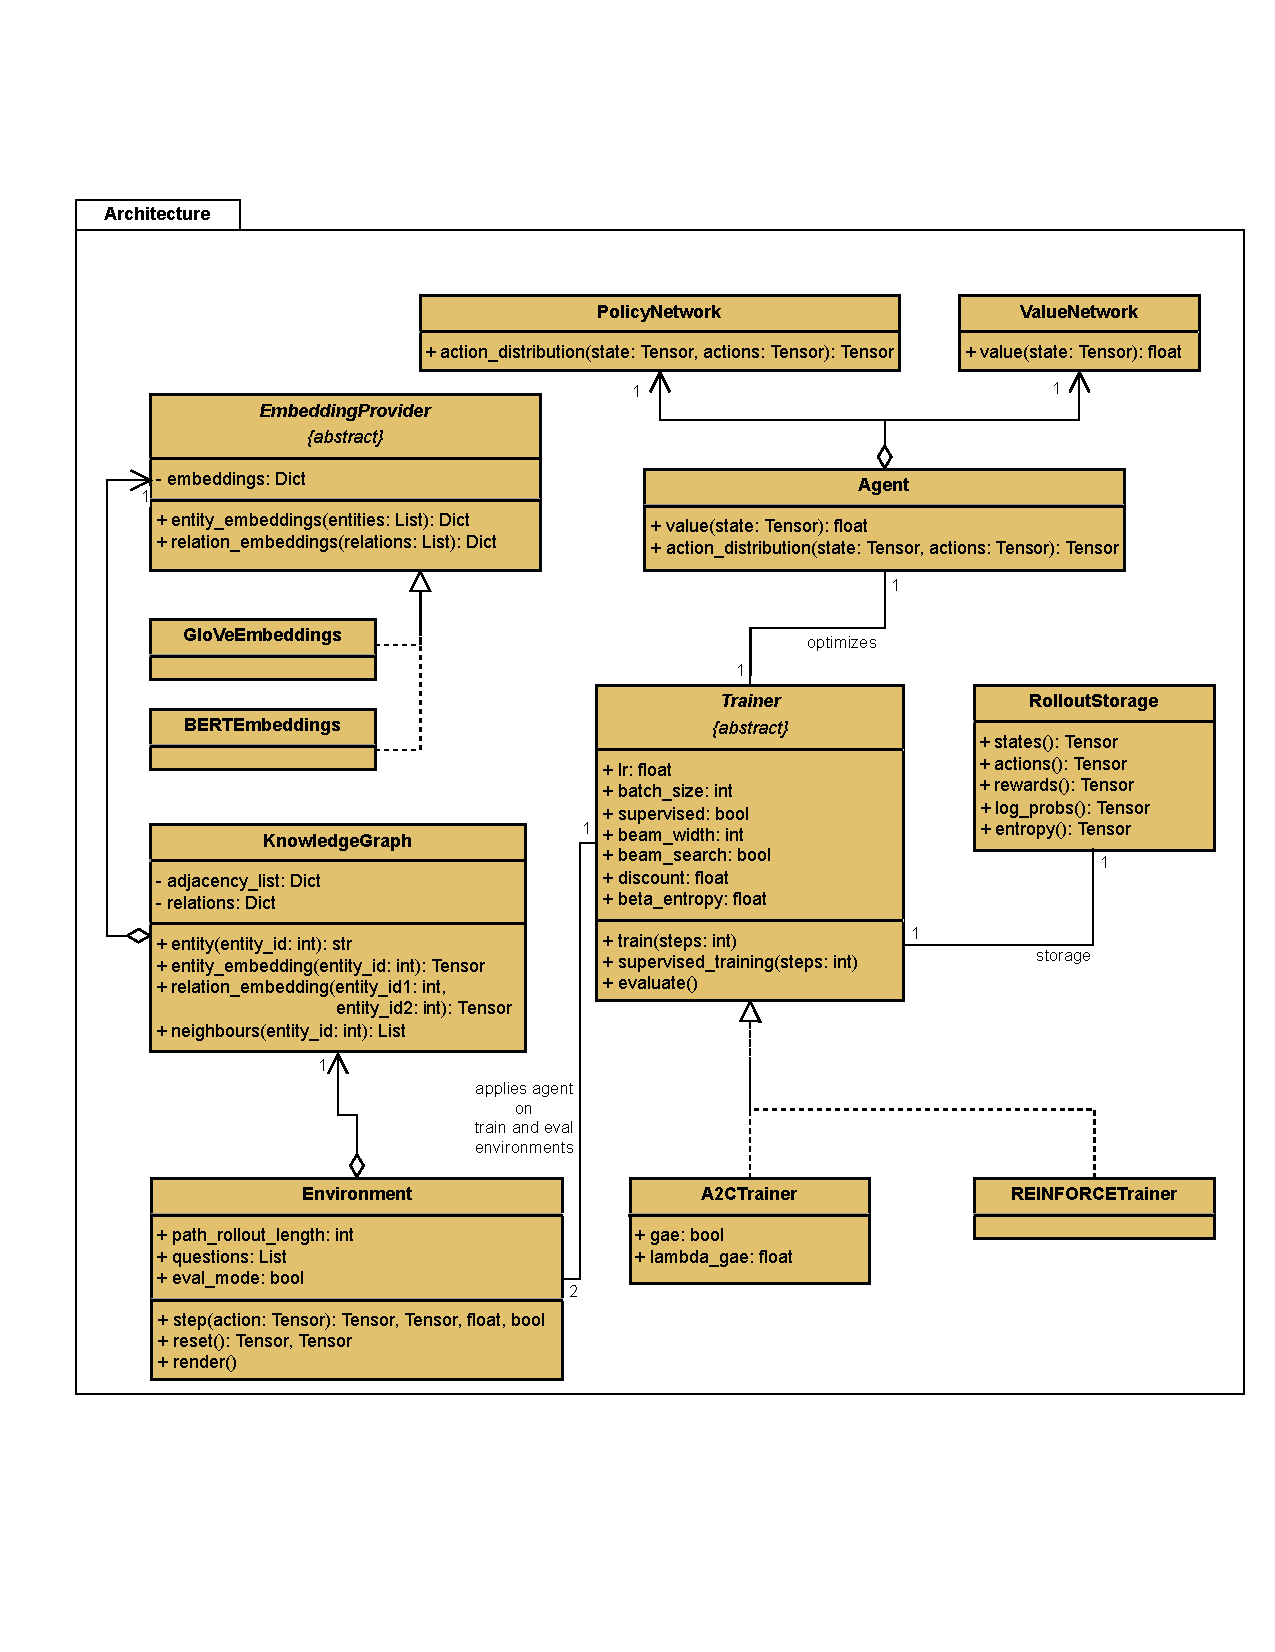
\includegraphics[clip, trim=0cm 4cm 0cm 2cm, width=1.15\textwidth]{figures/implementation}
	\caption{UML-Diagram depicting the architecture of our implementation. It shows the most important 
	classes, including the Trainer, Agent, and Environment, and how they interact with each other. For brevity, not 
	all parameters or methods are shown. Therefore, this figure should only provide a high-level overview. For the complete picture, 
	we provide an open-source implementation at: \\ \url{https://github.com/LukasBluebaum/Master_Thesis}}
	\label{fig:implementation}
  \end{figure}
% !TEX root = my-thesis.tex
%

\chapter{Evaluation}
\label{ch:evaluation}
In this chapter, we present the evaluation of our reinforcement learning
agent for causal question answering.
To start, we provide an overview of the used datasets, discuss
 the baselines that we used for comparison, and introduce the applied evaluation measures.
 Following this, we discuss parameter settings and further implementation details like 
 framework versions and the hardware used for training.
Afterward, we compare our agent to two baselines on the binary causal 
question answering task. Next, we conduct an ablation analysis 
to evaluate the effectiveness of the different parts of our approach.
Similarly, we showcase several experiments to analyze the impact of 
supervised learning and different decoding techniques.
Finally, we conclude this section by providing a few example paths found by 
our agent.


\section{Datasets}
\label{sec:datasets}
As shown in Section~\ref{subsec:causal-questions}, only one of the ten 
datasets from CausalQA~\cite{Bondarenko2022CausalQA} contained a larger number
of binary causal questions. Thus, we used the extracted questions from MS MARCO~\cite{Nguyen2016MSMARCO} as
one dataset and added SemEval~\cite{Hendrickx2010SemEval, SharpCausalQAEmbeddings2016}
as a second dataset. SemEval was curated by Sharp et al.~\cite{SharpCausalQAEmbeddings2016} by
selecting a subset of 1730 word pairs from the semantic relation classification 
benchmark SemEval 2010 Task 8~\cite{Hendrickx2010SemEval}.
Among the 1730 word pairs, there are 865 causal pairs and 865 non-causal pairs.

\begin{table}
\caption{Number of questions for training, validation, and testing for the MS MARCO~\cite{Nguyen2016MSMARCO}
and SemEval~\cite{SharpCausalQAEmbeddings2016} datasets. The ``|Effective Train|'' column shows the number of questions 
the agent has available for learning.}
\label{table-evaluation-datasets}
\centering
\begin{tabular}{lcccc} 
			\toprule
			\textbf{Dataset} & \textbf{|Train|} & \textbf{|Validation|} & \textbf{|Test|} & \textbf{|Effective Train|}\\
			\toprule
		   MS MARCO & 2169 & 241 & 263 & 1350 \\
		   SemEval & 1384 & 173 & 173 & 812 \\
			\bottomrule
\end{tabular}
\end{table}

Table~\ref{table-evaluation-datasets} shows the number of training, validation, and test questions for both
datasets. For SemEval, we randomly selected 10\% for validation and 
10\% for testing. For MS MARCO, we used the original validation set for testing and randomly
selected 10\% from the training set for validation. We optimized hyperparameters 
on the validation sets and then retrained using the combined training and validation sets.

The ``|Effective Train|'' column shows the number of questions available
for learning when combining the training and validation sets. As discussed in 
Section~\ref{sec:approach-description}, we only train on positive causal questions,
so we remove the negative causal questions during training. Additionally, we have to 
remove the questions from the training set where cause or effect cannot 
be found in CauseNet. Finally, that leaves us with 1350 questions for MS MARCO and 812 questions
for SemEval.

\section{Baselines}
\label{sec:baselines}

We compare our agent with two baselines: a breadth-first search (BFS) on CauseNet
 and the question answering system UnifiedQA-v2~\cite{Khashabi2020UnifiedQA, Khashabi2022UnifiedQA2}.
 The CauseNet paper~\cite{Heindorf2020Causenet} already used a BFS to estimate
 the recall of the graph. While they only considered paths up to length two, we 
 extended their implementation and added support for paths of arbitrary length.
 As done for our agent, we link the cause and effect of each question  
 to the graph using exact string matching. Afterward, BFS tries to find a path between cause 
 and effect to answer the question.
 
 BFS serves as a strong baseline and an upper limit on performance in certain circumstances.
 However, it should be noted that BFS can only be applied to binary causal questions. 
 Our agent only supports binary questions as proof of concept, but there are straightforward extensions to open-ended questions, as discussed in Chapter~\ref{ch:discussion}.
 For a given path length constrained, the BFS performs an exhaustive search and can represent an 
 upper limit on performance, with one exception.
 The exception is the potential introduction of false positives through inverse edges and errors in CauseNet.
 For example, assume we have a binary causal question~\textit{``Does X cause Y?''} 
 for which a causal relation only holds in the opposite direction, such that $Y$ causes $X$.
 Through the introduction of inverse edges, the BFS might find a path between the two and erroneously answer ``yes''.
 Similarly, if CauseNet contains an error and indicates that $X$ causes $Y$, the BFS will also provide an incorrect answer.
 While the BFS will always make these mistakes,\footnote{Assuming the false positives exist in CauseNet and can be found under the given path length constraint.} the agent 
 prunes the search space and can learn to avoid them.
 We summarize the implications of inverse edges in Chapter~\ref{ch:discussion}.

As a second baseline, we use UnifiedQA-v2~\cite{Khashabi2020UnifiedQA, Khashabi2022UnifiedQA2}. 
UnifiedQA-v2 is a text-to-text language model based on the T5 architecture~\cite{Raffel2020T5}
and achieved state-of-the-art performance on multiple datasets.
It was pre-trained on 20 question answering datasets of different formats, including extractive 
and abstractive question answering, multiple choice, and yes/no questions.
We chose UnifiedQA-v2 because it was used by CausalQA~\cite{Bondarenko2022CausalQA} for their 
evaluation, from which we extracted the binary causal questions.

We could not include the causal question answering approaches from related work 
because they are not open source, except for the approach by Kayesh et al.~\cite{KayeshCausalTransfer2020}. 
However, Kayesh et al. only released the code for training without the datasets and pre-trained models, so it was not possible for us to use their approach.
Similarly, the reinforcement learning-based approaches we encountered were either 
developed for different tasks~\cite{Kaiser2021Reinforcement}, had no available code~\cite{Qiu2020Stepwise}, 
or were designed for graphs with multiple relation types rather than 
the single relation type found in CauseNet~\cite{Das2018Minerva, Lin2020RewardShaping}.

\section{Evaluation Measures}
\label{sec:measures}
We evaluated our agent using standard binary classification measures: accuracy, $F_1$-score, 
precision, and recall. Precision represents the fraction of correct positive predictions, and recall 
represents the fraction of positive examples that were correctly predicted.

\begin{equation}
	Precision = \frac{TP}{TP + FP} \ \ \ \ \ \ \ Recall = \frac{TP}{TP + FN}
\end{equation}

Subsequently, the $F_1$-Score represents the harmonic mean of precision and recall, 
while
accuracy represents the fraction of correct predictions among all predictions.

\begin{equation}
	F_1\text{-}Score = 2\frac{precision \cdot recall}{precision + recall}
\end{equation}

\begin{equation}
	Accuracy = \frac{TP + TN}{TP + FP + FN + TN}
\end{equation}

Note that, at inference time, the accuracy is equal to the normalized reward of the agent.
During inference, the reward is always 0 or 1 since there is no cumulative reward 
calculation or reward shaping. Specifically, the agent receives a reward of 1 if the answer
is correct, which is defined as the agent finding a path when the causal 
relationship holds or not finding a path when the causal relationship does not hold. Conversely, the agent receives
a reward of 0 if the answer is incorrect. Thus, summing the rewards over all questions and 
dividing by the number of questions is equal to the accuracy.  


\section{Experimental Setup}
\label{sec:impl-details}

\begin{table}
\centering
\caption{The parameter configurations and the ranges we tested during hyperparameter optimization.
		 They are divided into general deep learning parameters, general reinforcement learning parameters,
		 and the parameters that are specific to our approach. This should not be a definite categorization, e.g., there are many 
		 other approaches which also use beam search, it is just provided to give a better overview.
		 }
\label{table-parameters}
\begin{tabular}{lrr} 
			\toprule
			\textbf{Parameter} & \textbf{Settings} & \textbf{Settings Sweeps}\\
			\midrule
			\textbf{General} & \\
			Learning Rate & 1e-4 & \{1e-3, 1e-4, 3e-4, 5e-5\}  \\ 
			Batch Size &  128  & \{16, 32, 64, 128\} \\
			Gradient Norm Clipping &  0.5 & \{0.5\}\\
			Hidden Dimension $h$ &  2048 & \{2048\}\\
			Seed &  42 & \{42\} \\
			Training Steps & 2000 & \{2000\}  \\ 
			\midrule
			\textbf{General Reinforcement Learning} & \\
			Discount $\gamma$ & 0.99 & \{0.9, 0.99, 1.0\}  \\
			GAE lambda $\lambda$ & 0.95 & \{0.95, 0.99, 1.0\} \\
			Entropy Weight $\beta$ & 0.01 & \{0.01, 0.05, 0.1\} \\
			\midrule
			\textbf{Specific to Our Approach} & \\
			Beam Width & 50 & \{1, 5, 10, 50\} \\
			Path Rollout Length Training & 3 & \{2, 3\} \\
			Path Rollout Length Evaluation & 3 & \{2, 3\} \\
			Supervised Ratio $\alpha$ & 0.8 & \{0.2, 0.4, 0.6, 0.8, 1.0\}  \\
			Supervised Steps & 300 & \{100, 200, 300\}  \\
			Supervised Batch Size & 64  & \{32, 64\} \\
			Reward Shaping Weight $\omega$ & 0.0 & \{0.0, 0.1, 0.5, 1.0\}  \\
			\bottomrule
\end{tabular}
\end{table}
In the following, we discuss the experimental setup for our agent, including the setup 
of the baselines, hyperparameter optimizations, and further implementation details.
The agent is configured with supervised learning at the start and uses the A2C 
algorithm together with beam search during inference time. Furthermore, inverse edges are 
added to CauseNet.
However, we did not include the reward shaping in the general configuration since 
it did not increase performance.
We further discuss the reward shaping in the ablation study in Section~\ref{sec:ablation-study}.

Table~\ref{table-parameters} presents the configurations for the experiments' parameters, including the ranges for hyperparameter sweeps.
For each dataset, we optimized the 
parameters on the validation set and retrained on the combined training and 
validation set afterward. The table shows the configurations for MS MARCO, whereas SemEval differs 
in two cases: 1.0 for the supervised ratio $\alpha$ and 32 for the supervised batch size.
For the hyperparameter ranges, we selected common values from the literature and values 
 successfully used in prior works~\cite{Das2018Minerva, Lin2020RewardShaping, Peng2018Mimic}.
In the experiments below, we denote the agent with path rollout length 2 as 
Agent 2-Hop and path rollout length 3 as Agent 3-Hop. Following related work~\cite{Das2018Minerva, Qiu2020Stepwise}, we consider paths up to length 3. However, 
this can be extended in future work. Similarly, the BFS 
baseline is called CauseNet 1-Hop, CauseNet 2-Hop, or CauseNet 3-Hop.


For optimization, we used the AdamW~\cite{Loshchilov2019AdamW} optimizer, with the PyTorch default settings of
$\beta_1 = 0.9 $, $\beta_2 = 0.999$, and weight decay $0.01$.
Additionally, we apply gradient norm clipping~\cite{Pascanu2013Clip} with a value of $0.5$.
We initialized the weights of the LSTM via orthogonal initialization~\cite{Saxe2014Orthogonal} and 
the weights of the feedforward networks with the kaiming initialization~\cite{Kaming2015Init}.
Moreover, we used Python 3.8.16 and PyTorch 1.13.0 for our experiments.
For the UnifiedQA-v2~\cite{Khashabi2020UnifiedQA, Khashabi2022UnifiedQA2} baseline, we chose 
the \textit{allenai/unifiedqa-v2-t5-base-1363200} checkpoint, which is included in 
the HuggingFace Transformers framework~\cite{Wolf2020Transformers}.
Furthermore, we used CauseNet-Precision~\cite{Heindorf2020Causenet} for our 
experiments due to its smaller action space and higher precision compared 
to CauseNet-Full. In future work, we will experiment with CauseNet-Full, especially 
with the performance tradeoffs between the precision and recall orientations of the 
two graphs.

To embed the states and actions, we used GloVe embeddings~\cite{Pennington2014Glove} with a dimensionality of 300.
When an entity contained more than one word, we used the average of their embeddings. Similarly, for the 
questions and sentences, we used the average of the embeddings of their words. 
We experimented with embeddings computed from RoBERTa~\cite{Liu2019Roberta} and MPNet~\cite{Song2020MPNet} 
but did not see performance improvements. 
One disadvantage of using GloVe embeddings might be that not all occurring words have a 
corresponding embedding. However, this occurs only for around 1\% of the entities in CauseNet-Precision, and 
manual checks showed that these do not pose problems for the questions in our datasets.
For the reward shaping, we slightly adapted the implementation of Yasunaga et al.~\cite{Yasunaga2021QAGNN} 
for our task. As the language model, we used the \textit{roberta-large}~\cite{Liu2019Roberta} checkpoint
from the Huggingface Transformers framework~\cite{Wolf2020Transformers}.

All experiments were run on Noctua 2\footnote{\url{https://pc2.uni-paderborn.de/de/hpc-services/available-systems/noctua2}} on the Paderborn 
Center for Parallel Computing (PC$^2)$\footnote{\url{https://pc2.uni-paderborn.de/}} and Google Colab.
Accordingly, we used a number of different GPUs for our experiments, mainly  NVIDIA A100 
40GB, NVIDIA Tesla T4 16GB, and NVIDIA Tesla V100 16GB.


\section{Evaluation of our Reinforcement Learning Agent}
\label{sec:evaluation-approach}


\renewcommand{\tabcolsep}{6pt}
\begin{table}
\centering
\caption{Evaluation results of our agent on the MS MARCO and SemEval test sets compared to the BFS baseline and UnifiedQA-v2. The table reports the 
		accuracy: \textbf{A}, $F_1$-Score: $\mathbf{F_1}$, recall: \textbf{R}, precision: \textbf{P}, and the number of nodes \textbf{|Nodes|} that were visited.
		The results for UnifiedQA-v2 using the paths of the agent as context are denoted as \textit{UnifiedQA-v2 -- Context}. The results when combining two approaches by answering ``yes'' if at least one of them answers ``yes'' are denoted as \textit{UnifiedQA-v2 | CauseNet 3-Hop} and \textit{UnifiedQA-v2 | Agent 3-Hop}.
		}
\label{table-evaluation-msmarco}
\begin{tabular}{lccccr} 
			\toprule
			\multicolumn{6}{c}{\textbf{MS MARCO}}\\
			\midrule
			& \textbf{A} & \textbf{$\mathbf{F_1}$} & \textbf{R} & \textbf{P} & \textbf{|Nodes|}\\
			\midrule
			%Agent 1-Hop & 0.36 & & \\
			Agent 2-Hop & 0.460 & 0.562 & 0.408 & 0.901 & 6,774\\
			Agent 3-Hop & 0.529 & 0.648 & 0.511 & 0.884 & 7,034 \\
			\midrule
			CauseNet 1-Hop & 0.259 & 0.241 & 0.139 & 0.912 & 14,937 \\ 
			CauseNet 2-Hop & 0.494 & 0.612 & 0.471 & 0.875 & 454,126 \\ 
			CauseNet 3-Hop & 0.589 & 0.714 & 0.605 & 0.871 & 878,090\\ 
			\midrule
			UnifiedQA-v2 & 0.722 & 0.828 & 0.789 & 0.871 & -- \\
			UnifiedQA-v2 | CauseNet 3-Hop & 0.787 & 0.877 & 0.897 & 0.858 & --  \\
			UnifiedQA-v2 | Agent 3-Hop & 0.779 & 0.872 & 0.883 & 0.860 & -- \\
			UnifiedQA-v2 --- Context & 0.661 & 0.789 & 0.740 & 0.842 & --\\
			\midrule
			Majority Baseline (True) & 0.848  & 0.9177 & 1.000 & 0.848 & --\\
			\bottomrule
\end{tabular}
%\end{table}
%\begin{table}[t]
\label{table-evaluation-semeval}
\centering
\renewcommand{\tabcolsep}{6.47pt}
\hspace{-0.20cm}
%\caption{Evaluation SemEval.}
\begin{tabular}{lccccr} 
			\toprule
			\multicolumn{6}{c}{\textbf{SemEval}}\\
			\midrule
			& \textbf{A} & \textbf{$\mathbf{F_1}$} & \textbf{R} & \textbf{P} & \textbf{|Nodes|}\\
			\midrule
			%Agent 1-Hop & 0.36 & & \\
			Agent 2-Hop &  0.769 & 0.714 & 0.575 & 0.943 & 4,641\\
			Agent 3-Hop & 0.775 & 0.727 & 0.598 & 0.929 & 4,947\\
			\midrule
			CauseNet 1-Hop & 0.665 & 0.508 & 0.345 & 0.968 & 6,080 \\ 
			CauseNet 2-Hop & 0.815 & 0.787 & 0.678 & 0.937 & 270,779 \\ 
			CauseNet 3-Hop & 0.751 & 0.754 & 0.759 & 0.750 & 637,821\\ 
			\midrule
			UnifiedQA-v2 & 0.497 & 0.653 & 0.943 & 0.500 & --\\
			UnifiedQA-v2 | CauseNet 3-Hop & 0.520 & 0.677 & 1.000 & 0.512 & -- \\
			UnifiedQA-v2 | Agent 3-Hop & 0.520 & 0.675 & 0.989 & 0.512 & -- \\
			UnifiedQA-v2 --- Context & 0.566 & 0.651 & 0.805 & 0.547 & -- \\
			\midrule
			Majority Baseline (True) & 0.503 & 0.669 & 1.000 & 0.503 & -- \\
			\bottomrule
\end{tabular}
\end{table}
In Table~\ref{table-evaluation-msmarco}, we show the evaluation results of our agent on the MS MARCO and SemEval 
test sets. We compare our agent in the Agent 2-Hop and Agent 3-Hop configurations with the corresponding 
BFS configurations CauseNet 1-Hop, CauseNet 2-Hop, and CauseNet 3-Hop. Moreover, we compare the results 
to UnifiedQA-v2 and explore some combinations of approaches as described below.
The table displays the accuracy, $F_1$-Score, recall, precision,
and the number of visited nodes summed over all questions for each dataset. Note that the number of visited nodes is not applicable for the UnifiedQA-v2-based approaches and the majority baseline.

When comparing the results of our agent and BFS, we observe that the agent does not fully match the performance of BFS in most configurations.
For instance, in the 2-Hop case, the agent is slightly behind by around 0.03 accuracy on MS MARCO and around 0.05 accuracy on SemEval.
However, the agent achieves better precision for all configurations, particularly for the 3-Hop configuration on SemEval.
In that case, the results of BFS are worse in the 3-Hop setting compared to the 2-Hop setting due to the 
 introduction of many false positives through inverse edges.\footnote{The results of CauseNet 3-Hop on SemEval are improved when not using inverse edges. However, using inverse edges improves the results for all other configurations. Thus, we included them in the graph as they also improve the performance of our agent, as shown in the ablation study in Section~\ref{sec:ablation-study}.} 
As discussed in~\ref{sec:baselines}, inverse edges can lead to mistakes by potentially introducing false positives.
When going from 2 hops to 3 hops on SemEval, it is possible to reach more false positives than before. 
This is especially indicated by the reduced precision of CauseNet 3-Hop, i.e., the precision is now 0.75, down from 0.875 of CauseNet 2-Hop.

In contrast, the agent mitigates this problem by pruning the search space and avoiding paths leading to wrong answers, still achieving a precision of 0.929.
Therefore, the agent slightly improves the results when comparing the 2 hop and 3 hop configurations. Also, the agent performs better than 
BFS in the 3-Hop configuration on SemEval.
Overall, compared to BFS, our agent has several advantages:
(1) it can be extended to open-ended causal questions as discussed in Chapter~\ref{ch:discussion},
(2) it can to avoid false positives introduced by inverse edges and errors in CauseNet as shown above,
(3) it prunes the search space and
decreases the number of visited nodes by around 99\%, on average searching only 25-30 nodes per question.
In comparison, BFS searches approximately 1500 nodes per question with 2 hops and 3500 nodes per question with 3 hops.

Furthermore, the results of UnifiedQA-v2~\cite{Khashabi2020UnifiedQA, Khashabi2022UnifiedQA2} vary significantly between the two datasets. 
Specifically, UnifiedQA-v2 is better than our agent on MS MARCO and worse on SemEval.
This can be attributed to UnifiedQA-v2's tendency to answer with ``yes'' most of the time. 
In addition, the MS MARCO test set is heavily skewed towards positive questions (80\% positive, 20\% negative), whereas the SemEval test set is more balanced (50\% positive, 50\% negative).
Thus, the results of UnifiedQA-v2's are better on MS MARCO than on SemEval.
 UnifiedQA-v2's tendency to answer ``yes'' is also indicated by the high recall of 0.943 and low precision of 0.500 on SemEval.


Finally, we explored a few simple strategies to combine our agent or BFS with UnifiedQA-v2.
\textit{UnifiedQA-v2 | CauseNet 3-Hop} and \textit{UnifiedQA-v2 | Agent 3-Hop} answer with ``yes'' when at least one of the two approaches answers with ``yes''.
Both strategies increase accuracy on MS MARCO by around 0.02 and SemEval by around 0.06.
Indicating, that even though UnifiedQA-v2 answers with ``yes'' in most cases, it still misses some of the questions 
where ``yes'' is the correct answer.

Moreover, we tested the effectiveness of using paths learned by our agent as context for UnifiedQA-v2.
For a given question, we took the learned paths and extracted the original sentence of each relation on the path.
Subsequently, we concatenated the question with the sentences and provided the resulting text as input to UnifiedQA-v2.
The results are mixed, with a decrease in accuracy by 0.06 on MS MARCO and an increase in accuracy by 0.06 on SemEval.
The issue may be that the context provided by the agent can be misleading. For instance, as the agent is not perfect, it does not always find 
correct paths for ``yes'' questions. Thus, on MS MARCO, where a majority of questions are positive, the agent 
might mislead UnifiedQA-v2 to change correct ``yes'' answers to ``no'' erroneously. In contrast, on SemEval, where many more questions 
are negative, the agent helps UnifiedQA-v2 to correctly change wrong ``yes'' answers to ``no''.


%\include{tables/table-evaluation}


\section{Ablation Study}
\label{sec:ablation-study}

\begin{table}
\renewcommand{\tabcolsep}{3pt}
\centering
\caption{Results of the ablation study, where we compare different configurations of our approach. For each configuration, we 
either remove ($\mathbf{-}$) or add ($\mathbf{+}$) some component. The evaluation measures are 
abbreviated as follows: accuracy: \textbf{A}, $F_1$-Score: $\mathbf{F_1}$, recall: \textbf{R}, precision: \textbf{P}.}
\label{table-ablation}
	\begin{tabular}{lcccccccc} 
		\toprule
		& \multicolumn{4}{c}{\textbf{MS MARCO}} & \multicolumn{4}{c}{\textbf{SemEval}}  \\
		\cmidrule(lr{.6em}){2-5} \cmidrule(l{0.3em}){6-9}
		&\textbf{A} & \textbf{$\mathbf{F_1}$} & \textbf{R} & \textbf{P} & \textbf{A} & \textbf{$\mathbf{F_1}$} & \textbf{R} & \textbf{P}\\
		\midrule
		Agent 2-Hop & \textbf{0.460} & \textbf{0.562} & \textbf{0.408} & 0.901 & \textbf{0.769} & \textbf{0.714} & \textbf{0.575} & 0.943 \\ 
		\midrule
		$\mathbf{-}$ Beam Search & 0.293 & 0.306 &0.184 & \textbf{0.911} & 0.613 & 0.374 &0.230& \textbf{1.000} \\
		$\mathbf{-}$ Supervised Learning & 0.342 & 0.397 & 0.257 & 0.891 & 0.682 & 0.538 & 0.369 & \textbf{1.000} \\
		$\mathbf{-}$ Actor-Critic & 0.441 & 0.539 & 0.386 & 0.896 & 0.740 & 0.657 &0.494& 0.977 \\
		$\mathbf{-}$ Inverse Edges & 0.422 & 0.513 &0.359& 0.899 & 0.740 & 0.651 & 0.483 & \textbf{1.000} \\
		$\mathbf{+}$ Reward Shaping (0.1) & 0.449 & 0.548 & 0.395 & 0.898 & 0.757 & 0.691 & 0.540 & 0.959 \\
		$\mathbf{+}$ Reward Shaping (1.0) & 0.403 &0.489 & 0.336 & 0.893 & \textbf{0.769} & 0.706 & 0.552 & 0.980 \\
		\bottomrule
	\end{tabular}
\end{table}

In our ablation study in Table~\ref{table-ablation}, we investigate the performance impact of the different components 
of our approach. Accordingly, we try out the following configurations: (1) without supervised 
learning, i.e., we run Algorithm~\ref{alg:algorithm} directly and train the policy and value network with 
policy gradients from scratch, (2) without Actor-Critic, we remove the critic and only run the 
REINFORCE algorithm using the Monte-Carlo return as described in Section~\ref{subsec:rl}, (3) we remove the beam search and use 
greedy decoding to only sample the most probable path, (4) without inverse edges in the graph, 
(5) with the extra reward signal through the reward shaping technique as explained in Section~\ref{sec:reward-shaping}.
Hence, a $-$ indicates the removal of some component, while a $+$ indicates the addition of a component.
Each configuration uses Agent 2-Hop with the settings described in Section~\ref{sec:impl-details}.

Overall, beam search has the biggest impact on performance. When beam search 
is exchanged for greedy decoding, the accuracy drops from 0.460 to 0.293 on 
MS MARCO and from 0.769 to 0.613 on SemEval. As further analysis of the decoding techniques shows (Section~\ref{sec:decoding-analysis}), 
the accuracy keeps increasing with a higher beam width.
Notably, greedy decoding slightly increases the precision on MS MARCO and does reach a precision of 1.0 compared 
to the 0.943 of beam search on SemEval.
Thus, the number of false positives decreases when only using the most probable path found by greedy decoding.
Moreover, supervised learning has the second highest impact. We analyze the effectiveness of supervised learning in Section~\ref{sec:evaluation-supervised} in more detail.

The Actor-Critic algorithm only has a minor 
impact with a difference of around 0.02-0.03 points accuracy on both datasets. Note that the $\lambda$-returns~\cite{Sutton1998RL} and GAE~\cite{Schulman2016GAE}, which we use in our Actor-Critic implementation, 
rely on multi-step returns and a bootstrap estimate via the value function to reduce the variance. At the moment, we only consider shorter paths 
of lengths 2 and 3, which might limit their impact. For this reason, we hypothesize that the impact 
compared to REINFORCE could further increase with longer paths.
Additionally, the removal of inverse edges from the graph results in a slight decrease in overall performance but an increase in precision on the SemEval dataset to 1.0. 
That is because the removal of inverse edges reduces the probability of finding false positives, as discussed in Section~\ref{sec:evaluation-approach}.

Next, we discuss the impact of reward shaping. 
Recall that the reward shaping introduces the $\omega$ hyperparameter used to weigh the auxiliary rewards when the search is unsuccessful.
During hyperparameter optimization, we tried a range of settings between 0.0 and 1.0.
We show two configurations in Table~\ref{table-ablation}, one for a smaller weight (0.1) and one for a
larger weight (1.0). 
As $\omega$ increases, the accuracy on the MS MARCO dataset decreases.
Smaller $\omega$ either decrease the performance slightly or make no difference at all.
In contrast, on SemEval, the configuration of $\omega$ is less impactful, e.g., with $\omega = 1.0$, the accuracy is identical to the standard configuration.
Notably, on SemEval, increasing $\omega$ also increases the precision.
Overall, introducing the language model score as an auxiliary reward signal 
is not beneficial in its current form.
Hence, this reward shaping technique requires further investigation and improvements 
in future work.

\section{Effects of Supervised Learning}
\label{sec:evaluation-supervised}

Below, we investigate the effects of supervised learning in more detail. To recall, the 
objective of supervised learning was to bootstrap the agent with expert demonstrations to 
better deal with the large action space. Thus, the expert demonstrations should 
leave the agent with a strong foundation for further improvement.

Therefore, we compare the performance of the agent when using different numbers of supervised 
training steps. Figure~\ref{figure-supervised} shows the accuracy of the agent on the SemEval~\cite{SharpCausalQAEmbeddings2016} test set
depending on the number of reinforcement learning training steps. Each of the three runs was 
bootstrapped with a different number of supervised training steps. Thus, at step 0, we can see the accuracy 
directly after supervised learning without any training via reinforcement learning.
We observe that the run with 100 steps is significantly worse than the runs with 200 and 300 steps.
It starts at around 0.67 directly after supervised learning and increases to around 0.72.
Whereas the difference between 200 to 300 steps is already a lot smaller. Both start between 0.72 and 0.73 and follow 
similar trajectories afterward to reach an accuracy of around 0.76 after 2000 reinforcement learning steps.
To maintain the clarity of the figures, we did not include a run with 400 steps, but the trend of diminishing returns 
on the number of supervised steps continues. 
This suggests that increasing the number of supervised steps beyond 300 does not improve performance.
Likewise, we observed similar results on the MS MARCO~\cite{Nguyen2016MSMARCO} dataset.

\begin{figure}
\centering
\begin{tikzpicture}
	\begin{axis}
		[	%legend pos=outer north east,
			legend cell align={left},
			legend style={legend pos=south east},
			xlabel=steps,
			ylabel=accuracy,
			grid=major,
			xtick={0, 20, 40, 60, 80, 100, 120, 140, 160, 180, 200},
			xticklabels={0, 200 , 400, 600, 800, 1000, 1200, 1400, 1800, 1900, 2000},
			ytick={0.66, 0.68, 0.70, 0.72, 0.74, 0.76, 0.78, 0.80},
			yticklabels={0.66, 0.68, 0.70, 0.72, 0.74, 0.76, 0.78, 0.80},
			xmin=0,
			xmax=200,
			ymin=0.66,
			ymax=0.80,
			width=14cm,
			height=9cm]
		%\addplot[mark=none, tab20darkgreen, very thick] table [x=Step, y=r_semeval_400_1.0_32_5000_ff - accuracy, col sep=comma] {data/supervised_accuracy.csv};
		%\addlegendentry{400 Steps}
		\addplot[mark=none, tab20darkred, very thick] table [x=Step, y=r_semeval_300_1.0_32_5000_ff - accuracy, col sep=comma] {data/supervised_accuracy.csv};
		\addlegendentry{300 Steps}
		\addplot[mark=none, tab20darkblue, very thick] table [x=Step, y=r_semeval_200_1.0_32_5000_ff - accuracy, col sep=comma] {data/supervised_accuracy.csv};
		\addlegendentry{200 Steps}
		\addplot[mark=none, tab20darkorange, very thick] table [x=Step, y=r_semeval_100_1.0_32_5000_ff - accuracy, col sep=comma] {data/supervised_accuracy.csv};
		\addlegendentry{100 Steps}
	\end{axis}
\end{tikzpicture}
	\caption{The figure shows the accuracy of the agent on the SemEval test set depending on the number of reinforcement learning training steps. Each 
			run was bootstrapped with a different number of supervised training steps. Step 0 shows the performance directly after supervised learning.}
	\label{figure-supervised}
\end{figure}

\begin{figure}[ht]
	\begin{minipage}{.45\linewidth}
	  \centering
\begin{tikzpicture}
	\hspace{-1.5cm}
	\begin{axis}
		[	%legend pos=outer north east,
			legend cell align={left},
			legend style={legend pos=north west},
			xlabel=steps,
			ylabel=|paths|,
			%ylabel shift = 0.1 pt,
			scaled y ticks = false,
			grid=major,
			xtick={0, 50, 100, 150, 200},
			xticklabels={0, 500, 1000, 1500, 2000},
			ytick={0, 20000, 40000, 60000, 80000},
			yticklabels={0, 20000, 40000, 60000, 80000},
			xmin=0,
			xmax=200,
			ymin=0,
			ymax=80000,
			width=8cm,
			height=8cm]
		%\addplot[mark=none, tab20darkgreen, very thick] table [x=Step, y=r_semeval_400_1.0_32_5000_ff - unique_paths, col sep=comma] {data/supervised_paths.csv};
		%\addlegendentry{400 Steps}
		\addplot[mark=none, tab20darkred, very thick] table [x=Step, y=r_semeval_300_1.0_32_5000_ff - unique_paths, col sep=comma] {data/supervised_paths.csv};
		\addlegendentry{300 Steps}
		\addplot [mark=none, tab20darkblue, very thick]table [x=Step, y=r_semeval_200_1.0_32_5000_ff - unique_paths, col sep=comma] {data/supervised_paths.csv};
		\addlegendentry{200 Steps}
		\addplot [mark=none, tab20darkorange, very thick]table [x=Step, y=r_semeval_100_1.0_32_5000_ff - unique_paths, col sep=comma] {data/supervised_paths.csv};
		\addlegendentry{100 Steps}
		\addplot [mark=none, tab20darkgreen, very thick]table [x=Step, y=r_semeval_no_super_5000_ff - unique_paths, col sep=comma] {data/supervised_paths.csv};
		\addlegendentry{0 Steps}
	\end{axis}
\end{tikzpicture}
	\end{minipage}
	\hspace*{0.7cm}
	\begin{minipage}{.45\linewidth}
	  \centering
\begin{tikzpicture}
	\begin{axis}
		[	%legend pos=outer north east,
			legend cell align={left},
			legend style={legend pos=north east},
			xlabel=steps,
			ylabel=entropy,
			grid=major,
			xtick={0, 50, 100, 150, 200},
			xticklabels={0, 500, 1000, 1500, 2000},
			ytick={0.0, 0.5, 1.0, 1.5, 2.0, 2.5, 3.0, 3.5},
			yticklabels={0.0, 0.5, 1.0, 1.5, 2.0, 2.5, 3.0, 3.5},
			xmin=0,
			xmax=200,
			ymin=0.0,
			ymax=3.5,
			width=8cm,
			height=8cm]
		%\addplot[mark=none, tab20darkgreen, very thick] table [x=Step, y=r_semeval_400_1.0_32_5000_ff - entropy, col sep=comma] {data/supervised_entropy.csv};
		%\addlegendentry{400 Steps}
		\addplot[mark=none, tab20darkred, very thick] table [x=Step, y=r_semeval_300_1.0_32_5000_ff - entropy, col sep=comma] {data/supervised_entropy.csv};
		\addlegendentry{300 Steps}
		\addplot [mark=none, tab20darkblue, very thick]table [x=Step, y=r_semeval_200_1.0_32_5000_ff - entropy, col sep=comma] {data/supervised_entropy.csv};
		\addlegendentry{200 Steps}
		\addplot [mark=none, tab20darkorange, very thick]table [x=Step, y=r_semeval_100_1.0_32_5000_ff - entropy, col sep=comma] {data/supervised_entropy.csv};
		\addlegendentry{100 Steps}
		\addplot[mark=none, tab20darkgreen, very thick] table [x=Step, y=r_semeval_no_super_5000_ff - entropy, col sep=comma] {data/supervised_entropy.csv};
		\addlegendentry{0 Steps}
	\end{axis}
\end{tikzpicture}
	\end{minipage}
	\caption{The figure shows the number of unique paths explored during reinforcement learning training on the left and the mean entropy of the action distribution of the policy network on the right. Each run was bootstrapped with a different number of supervised training steps.}
	\label{figure-supervised-entropy}
  \end{figure}
Moreover, Figure~\ref{figure-supervised-entropy} illustrates the number of unique paths explored during training on the left and
the mean entropy of the action distribution of the policy network on the right. Notably, with an increasing number 
of supervised steps, the entropy of the policy network drops significantly.
Hence, the number of explored paths during reinforcement learning also decreases as shown on the left in Figure~\ref{figure-supervised-entropy}.
These findings indicate that supervised learning
effectively establishes a strong foundation for the reinforcement learning agent.
For example, an agent trained with 300 supervised steps only explores $21.6\%$ of the paths of 
an agent without any supervised steps at the start.
Accordingly, the agent trained with 300 supervised steps can exploit the knowledge acquired during supervised learning to follow better paths.
In contrast, the agent trained without any supervised learning steps requires more exploration and fails to achieve the same performance, 
as shown in Table~\ref{table-ablation}.


%\include{figures/supervised}


\section{Decoding Analysis}
\label{sec:decoding-analysis}

In the following, we investigate the effects of different beam widths on the MS MARCO test set. We experimented with 
beam widths of 1, 5, 10, and 50 and present the results in Figure~\ref{figure-beam-search-whole-path}. In these experiments, we did not apply 
supervised learning at the beginning to focus solely on the effects of beam width settings. Additionally, 
we increased the training steps from 2000 to 4000 because, without supervised learning, there is still 
some progress after 2000 steps.

In general, as the beam width increases, accuracy also increases. For example, the difference between a width of 1 and a width of 50 is 0.09 points accuracy after 2000 steps.
The exception is between widths of 5 and 10, which reach the same accuracy after 2000 steps and have similar curves.
In Section~\ref{sec:search}, we noted that beam search can be viewed as an interpolation between greedy decoding and BFS.
Therefore, if the beam width is set too high, the task may become too easy as the agent performs an exhaustive search, disregarding runtime considerations for a moment.
We can already observe this effect when looking at the accuracy immediately after initialization at step 0.
As the beam width increases, the accuracy without any learning also increases slightly, e.g., for widths of 10 and 50 from 0.18 to 0.21.
However, the increases are minor, and even beam width 50 only starts at 0.21 and still has a lot of learning progress afterward.
Additionally, the performance from width 50 does not reach the performance with supervised learning or the performance of the BFS.
This suggests that a beam width of 50 is still reasonable, and we could have also used a higher beam width, like 100, for our experiments. 

Our standard setup evaluates the paths by checking if any of their entities match the target entity. 
However, in Section~\ref{sec:env}, we introduced the \textit{STAY} action and trained the agent 
 on path rollouts of the same length.
 Hence, when the agent reaches the target entity, it should have learned to use the \textit{STAY} action and stop advancing.
Therefore, we investigate whether the agent behaves accordingly in Figure~\ref{figure-beam-search-final-node}.

The runs in Figure~\ref{figure-beam-search-final-node} use the same setup as those in Figure~\ref{figure-beam-search-whole-path}, 
except that we only compare the last node on each path to the target entity.
This setup allows us to determine whether the agent always stays at the target entity or sometimes walks over it.
The figures illustrate that there is a slight difference between the two setups.
In case we only check the last node, the accuracy after 4000 steps is always around 0.01-0.02 points accuracy lower when comparing the runs with the same beam width.
While the difference is small, this suggests that the agent does not always stop when necessary.
As an illustration, we provide an example in Section~\ref{sec:path-analysis}.


%\begin{figure}
\centering
\begin{tikzpicture}
	\begin{axis}
		[	%legend pos=outer north east,
			legend cell align={left},
			legend style={legend pos=south east},
			xlabel=steps,
			ylabel=accuracy,
			grid=major,
			xtick={0, 40, 80, 120, 160, 200, 240, 280, 320, 360, 400},
			xticklabels={0, 400, 800, 1200, 1600, 2000, 2400, 2800, 3200, 3600, 4000},
			ytick={0.1, 0.15, 0.2, 0.25, 0.3, 0.35, 0.4},
			yticklabels={0.1, 0.15, 0.2, 0.25, 0.3, 0.35, 0.4},
			xmin=0,
			xmax=400,
			ymin=0.1,
			ymax=0.4,
			width=14cm,
			height=8cm]
		\addplot [mark=none, tab20darkgreen, very thick]table [x=Step, y=r_msmarco_bm_50_5000_ff - accuracy, col sep=comma] {data/beam_path_inverse.csv};
		\addlegendentry{Width: 50}
		\addplot [mark=none, tab20darkorange, very thick]table [x=Step, y=r_msmarco_bm_10_5000_ff - accuracy, col sep=comma] {data/beam_path_inverse.csv};
		\addlegendentry{Width: 10}
		\addplot [mark=none, tab20darkblue, very thick]table [x=Step, y=r_msmarco_bm_5_5000_ff - accuracy, col sep=comma] {data/beam_path_inverse.csv};
		\addlegendentry{Width: 5}
		\addplot[mark=none, tab20darkred, very thick] table [x=Step, y=r_msmarco_bm_1_5000_ff - accuracy, col sep=comma] {data/beam_path_inverse.csv};
		\addlegendentry{Width: 1}
	\end{axis}
\end{tikzpicture}
	\caption{Accuracy on the MS MARCO test set depending on the number of reinforcement learning training steps. Each run uses a different beam width and our standard setup, where we compare all entities on the paths to the target entity. 
			 }
	\label{figure-beam-search-whole-path}
\end{figure}

\begin{figure}
\centering
\begin{tikzpicture}
	\begin{axis}
		[	%legend pos=outer north east,
			legend cell align={left},
			legend style={legend pos=south east},
			xlabel=steps,
			ylabel=accuracy,
			grid=major,
			xtick={0, 40, 80, 120, 160, 200, 240, 280, 320, 360, 400},
			xticklabels={0, 400, 800, 1200, 1600, 2000, 2400, 2800, 3200, 3600, 4000},
			ytick={0.1, 0.15, 0.2, 0.25, 0.3, 0.35, 0.4},
			yticklabels={0.1, 0.15, 0.2, 0.25, 0.3, 0.35, 0.4},
			xmin=0,
			xmax=400,
			ymin=0.1,
			ymax=0.4,
			width=14cm,
			height=8cm]
		\addplot [mark=none, tab20darkgreen, very thick]table [x=Step, y=r_msmarco_bm_50_no_5000_ff - accuracy, col sep=comma] {data/beam_final_inverse.csv};
		\addlegendentry{Width: 50}
		\addplot [mark=none, tab20darkorange, very thick]table [x=Step, y=r_msmarco_bm_10_no_5000_ff - accuracy, col sep=comma] {data/beam_final_inverse.csv};
		\addlegendentry{Width: 10}
		\addplot [mark=none, tab20darkblue, very thick]table [x=Step, y=r_msmarco_bm_5_no_5000_ff - accuracy, col sep=comma] {data/beam_final_inverse.csv};
		\addlegendentry{Width: 5}
		\addplot[mark=none, tab20darkred, very thick] table [x=Step, y=r_msmarco_bm_1_no_5000_ff - accuracy, col sep=comma] {data/beam_final_inverse.csv};
		\addlegendentry{Width: 1}
	\end{axis}
\end{tikzpicture}
	\caption{Accuracy on the MS MARCO test set depending on the number of reinforcement learning training steps. Each run uses a different beam width. The figure illustrates a slightly different setup, where we only compare the last node on each path to the target entity. }
	\label{figure-beam-search-final-node}
\end{figure}

\begin{figure}
\centering
\begin{tikzpicture}
	\begin{axis}
		[	%legend pos=outer north east,
			legend cell align={left},
			legend style={legend pos=south east},
			xlabel=steps,
			ylabel=accuracy,
			grid=major,
			xtick={0, 40, 80, 120, 160, 200, 240, 280, 320, 360, 400},
			xticklabels={0, 400, 800, 1200, 1600, 2000, 2400, 2800, 3200, 3600, 4000},
			ytick={0.1, 0.15, 0.2, 0.25, 0.3, 0.35, 0.4},
			yticklabels={0.1, 0.15, 0.2, 0.25, 0.3, 0.35, 0.4},
			xmin=0,
			xmax=400,
			ymin=0.1,
			ymax=0.4,
			width=14cm,
			height=8cm]
		\addplot [mark=none, tab20darkgreen, very thick]table [x=Step, y=r_msmarco_bm_50_5000_ff - accuracy, col sep=comma] {data/beam_path_inverse.csv};
		\addlegendentry{Width: 50}
		\addplot [mark=none, tab20darkorange, very thick]table [x=Step, y=r_msmarco_bm_10_5000_ff - accuracy, col sep=comma] {data/beam_path_inverse.csv};
		\addlegendentry{Width: 10}
		\addplot [mark=none, tab20darkblue, very thick]table [x=Step, y=r_msmarco_bm_5_5000_ff - accuracy, col sep=comma] {data/beam_path_inverse.csv};
		\addlegendentry{Width: 5}
		\addplot[mark=none, tab20darkred, very thick] table [x=Step, y=r_msmarco_bm_1_5000_ff - accuracy, col sep=comma] {data/beam_path_inverse.csv};
		\addlegendentry{Width: 1}
	\end{axis}
\end{tikzpicture}
	\caption{Accuracy on the MS MARCO test set depending on the number of reinforcement learning training steps. Each run uses a different beam width and our standard setup, where we compare all entities on the paths to the target entity. 
			 }
	\label{figure-beam-search-whole-path}
\end{figure}

\begin{figure}
\centering
\begin{tikzpicture}
	\begin{axis}
		[	%legend pos=outer north east,
			legend cell align={left},
			legend style={legend pos=south east},
			xlabel=steps,
			ylabel=accuracy,
			grid=major,
			xtick={0, 40, 80, 120, 160, 200, 240, 280, 320, 360, 400},
			xticklabels={0, 400, 800, 1200, 1600, 2000, 2400, 2800, 3200, 3600, 4000},
			ytick={0.1, 0.15, 0.2, 0.25, 0.3, 0.35, 0.4},
			yticklabels={0.1, 0.15, 0.2, 0.25, 0.3, 0.35, 0.4},
			xmin=0,
			xmax=400,
			ymin=0.1,
			ymax=0.4,
			width=14cm,
			height=8cm]
		\addplot [mark=none, tab20darkgreen, very thick]table [x=Step, y=r_msmarco_bm_50_no_5000_ff - accuracy, col sep=comma] {data/beam_final_inverse.csv};
		\addlegendentry{Width: 50}
		\addplot [mark=none, tab20darkorange, very thick]table [x=Step, y=r_msmarco_bm_10_no_5000_ff - accuracy, col sep=comma] {data/beam_final_inverse.csv};
		\addlegendentry{Width: 10}
		\addplot [mark=none, tab20darkblue, very thick]table [x=Step, y=r_msmarco_bm_5_no_5000_ff - accuracy, col sep=comma] {data/beam_final_inverse.csv};
		\addlegendentry{Width: 5}
		\addplot[mark=none, tab20darkred, very thick] table [x=Step, y=r_msmarco_bm_1_no_5000_ff - accuracy, col sep=comma] {data/beam_final_inverse.csv};
		\addlegendentry{Width: 1}
	\end{axis}
\end{tikzpicture}
	\caption{Accuracy on the MS MARCO test set depending on the number of reinforcement learning training steps. Each run uses a different beam width. The figure illustrates a slightly different setup, where we only compare the last node on each path to the target entity. }
	\label{figure-beam-search-final-node}
\end{figure}

\section{Inference Time}
\label{sec:inference time}

\begin{figure}[ht]
	\begin{minipage}{.45\linewidth}
	  \centering
\begin{tikzpicture}
	\hspace{-1.0cm}
	\begin{axis}
		[	%legend pos=outer north east,
			legend cell align={left},
			legend style={legend pos=north west},
			xlabel=beam width,
			ylabel=seconds,
			%ylabel shift = 0.1 pt,
			scaled y ticks = false,
			grid=major,
			xtick={1, 10, 20, 30, 40, 50},
			xticklabels={1, 10, 20, 30, 40, 50},
			ytick={0, 30, 60, 90, 120, 150, 180},
			ytick={0, 30, 60, 90, 120, 150, 180},
			extra x ticks={25},
			extra x tick labels={\textbf{MS MARCO}},
			extra x tick style={grid=none,ticks=major,ticklabel pos=right},
			xmin=1,
			xmax=50,
			ymin=0,
			ymax=180,
			width=8cm,
			height=8cm]
		\addplot[mark=none, tab20darkred, very thick] table [x=width, y=numbers, col sep=comma] {data/length2_msmarco.csv};
		\addlegendentry{Length: 2}
		\addplot [mark=none, tab20darkblue, very thick]table [x=width, y=numbers, col sep=comma] {data/length3_msmarco.csv};
		\addlegendentry{Length: 3}
	\end{axis}
\end{tikzpicture}
	\end{minipage}
	\hspace*{0.5cm}
	\begin{minipage}{.45\linewidth}
	  \centering
\begin{tikzpicture}
	\begin{axis}
		[	%legend pos=outer north east,
			legend cell align={left},
			legend style={legend pos=north west},
			xlabel=beam width,
			ylabel=seconds,
			grid=major,
			xtick={1, 10, 20, 30, 40, 50},
			xticklabels={1, 10, 20, 30, 40, 50},
			ytick={0, 30, 60, 90, 120, 150, 180},
			ytick={0, 30, 60, 90, 120, 150, 180},
			extra x ticks={25},
			extra x tick labels={\textbf{SemEval}},
			extra x tick style={grid=none,ticks=major,ticklabel pos=right},
			xmin=1,
			xmax=50,
			ymin=0,
			ymax=180,
			width=8cm,
			height=8cm]
		\addplot[mark=none, tab20darkred, very thick] table [x=width, y=numbers, col sep=comma] {data/length2_semeval.csv};
		\addlegendentry{Length: 2}
		\addplot [mark=none, tab20darkblue, very thick]table [x=width, y=numbers, col sep=comma] {data/length3_semeval.csv};
		\addlegendentry{Length: 3}
	\end{axis}
\end{tikzpicture}
	\end{minipage}
	\caption{Inference time in seconds for the test sets depending on the beam width and path rollout length. The figure on the left shows the time for the MS MARCO test set, and the figure on the right for the SemEval test set. The agent takes longer for MS MARCO in both cases because the MS MARCO test set contains 90 questions more compared to SemEval.}
	\label{figure-inference}
\end{figure}

Figure~\ref{figure-inference} illustrates the inference runtime for both test sets, depending on the beam width and path rollout length.
The left figure presents the runtime on the MS MARCO test set, while the right figure shows the runtime for the SemEval test set.
Note that the time measurements do not include the setup of the environment, such as the 
loading of the knowledge graph and embeddings.

The MS MARCO test set contains 263 questions, while the SemEval test set only contains 173 questions. As a result, the runtime for MS MARCO is longer in both cases.
For a beam width of 50, the inference on MS MARCO takes 52 seconds for path rollout length 2 and 174 seconds for path rollout length 3, resulting in a runtime per question of around 0.20 seconds and 0.66 seconds, respectively.
Also, on SemEval, the inference takes 36 (0.21) seconds and 97 (0.56) seconds, so the time per question is 
similar for both datasets.
We observe that when increasing the path rollout length from 2 to 3,
the runtime 
already increases by a factor of around 3.
However, there is much room for improvement in the current beam search implementation,
particularly regarding batching and memory movements between CPU and GPU.
Generally, we can make a trade-off between performance and runtime.
As the beam width decreases, runtime also decreases; for example, in the case of a beam width of 1, the runtime would be around 0.05 seconds per question.
However, this would also decrease the accuracy, as shown in Figure~\ref{figure-beam-search-whole-path}.

As illustrated in the plots, the beam width does not always increase the runtime.
While the beam width is an important factor for the runtime, there are other factors to consider.
For example, the runtime also depends on the degree of the nodes on the explored paths, as the beam search must consider each neighbor as a potential candidate.

\section{Examples}
\label{sec:path-analysis}

Lastly, we provide some examples that our agent found. In Table~\ref{table-examples},
we illustrate two examples of Agent 2-Hop and four examples of Agent 3-Hop.
Each example includes a cause and an effect together with a path between them. 
The arrows on the paths indicate whether the agent took the standard \textit{cause} edge, the \textit{STAY} action, or an inverse edge \textit{$cause^{-1}$}.

The paths learned by the agent can be used to follow the complete reasoning chain to examine 
the mechanisms of how a cause produces an effect. For example, the first path from Agent 3-Hop indicates that the 
bacterium \textit{helicobacter pylori} can lead to the development of \textit{peptic ulcer} disease, which can 
lead to \textit{vomiting}. The first examples for Agent 2-Hop and Agent 3-Hop demonstrate the agent's 
ability to utilize the \textit{STAY} action. In general, the usage of the \textit{STAY} action works
well in most cases. However, as shown in Section~\ref{sec:decoding-analysis}, there are some exceptions where the \textit{STAY} should have been used but was not.
An example can be seen in the last path for Agent 3-Hop in Table~\ref{table-examples}.
The agent should have stayed at \textit{flooding} but went ahead to \textit{landslides} and stayed there.

Moreover, the agent learned to use inverse edges to recover from mistakes. In the third example for Agent 3-Hop, the 
agent went one step too far, from \textit{constipation} to \textit{depression}, and used an inverse edge afterward to 
return to the \textit{constipation} entity.

\begin{table}
\centering
\caption{Some examples that our agent found. Each example consists of a cause, an effect, and a path between them. For each path, we indicate whether the agent used a normal \textit{cause} edge, the \textit{STAY} action, or an inverse edge \textit{$cause^{-1}$}.}
\label{table-examples}
\begin{tabular}{m{13cm} m{0.2cm}}
  \toprule
  \multicolumn{2}{c}{\textbf{Agent 2-Hop}} \\
  \midrule
   \vspace{0.2cm}
  \textbf{Cause:} stress \hspace{1cm} \textbf{Effect:} skin rashes &\\ 
   \vspace{0.2cm}
  \textbf{Path:} stress $\xRightarrow{\text{cause}}$ skin rashes $\xRightarrow{\text{\textit{STAY}}}$ skin rashes\vspace{0.2cm}\\
  \midrule
   \vspace{0.2cm}
  \textbf{Cause:} cigarettes \hspace{0.32cm} \textbf{Effect:} nausea &\\ 
   \vspace{0.2cm}
  \textbf{Path:} cigarettes $\xRightarrow{\text{cause}}$ cancer $\xRightarrow{\text{cause}}$ nausea\vspace{0.2cm}\\
  \bottomrule
  \toprule
  \multicolumn{2}{c}{\textbf{Agent 3-Hop}} \\
  \midrule
   \vspace{0.2cm}
  \textbf{Cause:} h.\ pylori \hspace{0.54cm} \textbf{Effect:} vomiting &\\ 
   \vspace{0.2cm}
  \textbf{Path:} h.\ pylori $\xRightarrow{\text{cause}}$ peptic ulcer disease $\xRightarrow{\text{cause}}$ vomiting $\xRightarrow{\text{\textit{STAY}}}$ vomiting \vspace{0.2cm}\\
  \midrule
   \vspace{0.2cm}
  \textbf{Cause:} Xanax \hspace{0.92cm} \textbf{Effect:} hiccups &\\ 
   \vspace{0.2cm}
  \textbf{Path:} xanax $\xRightarrow{\text{cause}}$ anxiety $\xRightarrow{\text{cause}}$ stress $\xRightarrow{\text{cause}}$ hiccups \vspace{0.2cm}\\
  \midrule
   \vspace{0.2cm}
  \textbf{Cause:} chocolate \hspace{0.39cm} \textbf{Effect:} constipation &\\ 
   \vspace{0.2cm}
  \textbf{Path:} chocolate $\xRightarrow{\text{cause}}$ constipation $\xRightarrow{\text{cause}}$ depression $\xRightarrow{\text{cause}^{-1}}$ constipation \vspace{0.2cm}\\
  \midrule
   \vspace{0.2cm}
  \textbf{Cause:} rainfall \hspace{0.80cm} \textbf{Effect:} flooding &\\ 
   \vspace{0.2cm}
  \textbf{Path:} rainfall $\xRightarrow{\text{cause}}$ flooding $\xRightarrow{\text{cause}}$ landslides $\xRightarrow{\text{\textit{STAY}}}$ landslides \vspace{0.2cm}\\
  \bottomrule
\end{tabular}
\end{table}

% !TEX root = my-thesis.tex
%

\chapter{Discussion \& Future Work}
\label{ch:discussion}

Below, we discuss a few points, like the addition of inverse edges and how our approach 
can be used to explain the answers to causal questions. Additionally, we talk 
about possible directions for future work. These include the extension 
to more causal question types, the usage of different causal knowledge graphs, and 
model-based reinforcement learning techniques.

\paragraph{Inverse Edges}
For CauseNet~\cite{Heindorf2020Causenet}, the addition of inverse edges implies that the agent can also 
walk from an effect to its cause. In general, their addition has a few benefits, 
like the possibility to undo wrong actions and to reach nodes that otherwise could not be 
reached under a given path length constraint. Conversely, they also introduce the possibility 
to make mistakes through false positives, as described in Section~\ref{sec:baselines}. While these mistakes 
will always happen for the BFS, 
our agent can minimize them by pruning the search space, as demonstrated in our experiments in Section~\ref{sec:evaluation-approach}.

Moreover, it might not always be clear that it makes sense to take an inverse edge in theory.
For example, given a question like \textit{``Does X cause Y?''}, we start the search at $X$.
If we take an inverse edge from an entity $Z$ to $Y$ at some point during the search, 
it does not directly follow that $X$ causes $Y$ in theory.
However, as our experiments show (Section~\ref{sec:ablation-study}), adding 
inverse edges improves performance in practice, so their benefits seem to outweigh the pitfalls.
This is in line with prior works that also added inverse edges to improve performance~\cite{Xiong2017DeePpath,Das2018Minerva}.

\paragraph{Explainability of Causal Questions}
Our approach has the advantage of not only being able to answer binary causal 
questions but also to provide post-hoc explanations. Although, this only holds 
for questions that were answered with ``yes'' because CauseNet~\cite{Heindorf2020Causenet} does not contain 
negative information. If the agent found no path or the cause or effect 
could not be found in CauseNet, we can only answer with ``no'' without additional explanation why the causal 
relation does not hold.
Additionally, errors in CauseNet may lead to incorrect answers and explanations. 
However, with a precision of 96\% in CauseNet-Precision~\cite{Heindorf2020Causenet}, such scenarios are rare.

As the examples in Section~\ref{sec:path-analysis} show, the paths found during 
inference can be used to follow the complete reasoning chain. Thus, we can inspect 
the paths to examine the specific mechanisms by which the cause produces the effect, potentially through a chain 
of multiple entities. Moreover, since the agent might find multiple paths between a cause and effect 
pair, we can showcase multiple ways in which the cause and effect are related.

Finally, we can use the additional meta-information that is part of each relation~\cite{Heindorf2020Causenet}.
For example, we can reference the original sentence from which the relation was extracted, which may provide additional insights. 
Furthermore, each relation contains the URL of the original web source, which we can check to verify the causal relations and receive further information.
In general, this is not possible with a language model like UnifiedQA~\cite{Khashabi2020UnifiedQA, Khashabi2022UnifiedQA2}. For example, for binary causal questions, 
it provides a ``yes'' or ``no'' answer, possibly with an explanation, but with no direct way to verify this claim.
Although, research is ongoing to enhance language models with the 
ability to cite their sources~\cite{Menick2022Cite}.


\paragraph{Additional Causal Question Types}
At the moment, our approach only supports binary causal questions. In the following, 
we discuss a straightforward extension to Cause-Effect question. In Section~\ref{subsec:causal-questions}, we defined
 Cause-Effect questions as questions like \textit{``What causes pneumonia?''}, i.e., questions that ask for the 
 cause of a given effect or vice versa. These questions only require changes at inference time and no changes at 
 train time.\footnote{During training, one minor difference is that we do not take the cause and effect from the question, but rather one from the question and the other from the answer.}

Contrary to binary causal questions, we no longer have to verify a given causal relation but search for a suitable entity.
Therefore, we need to change the decoding at inference time since we no longer know the entity we are looking for.
Thus, we introduce a majority voting approach. Given a question like \textit{``What causes pneumonia?''}, 
we still sample multiple paths from the agent. Next, we count the occurrence of the entities on these 
paths and select the one with the highest count as the answer. Alternatively, we can 
conduct the ranking by summing their probabilities on different paths. Moreover, we can also provide 
multiple answers by selecting the top n candidates.
Overall, this approach only requires minor changes to our current code base.
To answer more complex questions like \textit{``How does smoking cause cancer?''}, we can 
run the agent to answer the question as if it were a binary question and then use one of the possibilities for explanations described above.


\paragraph{Causal Knowledge Graphs}
Our approach is inherently limited by CauseNet.
If a question requires information not present in CauseNet, our agent cannot provide an answer.
A simple extension would be the introduction of additional graphs 
like Cause Effect Graph~\cite{Li2020CauseEffectGraph}. Cause Effect Graph is another 
large-scale causal knowledge graph that is very similar to CauseNet's structure.
Subsequently, we can apply the agent on each 
graph and answer with ``yes'' if one of them yields a result. Conversely, if we want to optimize for 
precision, we would require both to yield a result.

Another possible extension is the introduction of graphs like ATOMIC~\cite{Sap2019ATOMIC}.
CauseNet contains causal relations between concepts like cancer, smoking, pneumonia, or anemia.
In contrast, ATOMIC contains relations about commonsense reasoning in everyday life.
These relations are presented in the form of ``If-Event-Then-X'' patterns. For example, social interactions like 
if ``Person X makes Person Y a compliment'', then ``Person Y will feel good''~\cite{Sap2019ATOMIC}.
These different knowledge types can complement each other and allow the agent to answer a 
greater variety of causal questions. 


\paragraph{False Positives \& Negative Causal Questions}
In future work, we plan to investigate different ways to handle false positives during training and incorporate negative causal questions.
As discussed, inverse edges and errors in CauseNet can introduce false positives.
Currently, during training, these errors are treated as any other error, resulting in a reward of 0. 
However, it could be argued that these types of errors should be treated differently, such as by assigning a negative reward.
To incentivize the agent to ignore errors in CauseNet and only to take inverse edges when appropriate.
Additionally, we will explore mechanisms for incorporating negative causal questions into training.
In the current setup, we excluded them because CauseNet does not contain negative information~\cite{Heindorf2020Causenet}.

\paragraph{Model-Based Reinforcement Learning}
As discussed above, the transition function of the MDP is known and deterministic because it is entirely defined by the static graph~\cite{Shen2018MWalk}.
Thus, M-Walk~\cite{Shen2018MWalk} used a model-based reinforcement learning algorithm similar to AlphaGo Zero~\cite{Silver2017AlphaGoZero}.
A possible improvement could be to use MuZero~\cite{Schrittwieser2020Muzero}, a successor of AlphaGo Zero.
Particularly interesting might be Sampled MuZero~\cite{Hubert2021Sampled}, an extension to MuZero designed to deal 
with large and complex action spaces.


\paragraph{Runtime Improvements}
In future works, we will add parallelization to our framework to decrease the training time.
Typical A2C implementations use multiple workers in parallel to sample episodes. However, in our current 
implementation, we only use one worker. To improve the inference time, we can improve our beam 
search implementation regarding the usage of batches and memory movements between CPU and GPU.
Furthermore, we can apply improvements like switching from eager mode to graph mode in PyTorch.
% !TEX root = my-thesis.tex
%
\chapter{Conclusion}
\label{ch:conclusion}

In this thesis, we introduced a reinforcement learning approach to answer binary causal questions 
on a causal knowledge graph. We extended the setup of many prior approaches for reasoning tasks
via reinforcement learning on knowledge graphs~\cite{Xiong2017DeePpath, Das2018Minerva, Qiu2020Stepwise, Kaiser2021Reinforcement} by transitioning from the REINFORCE~\cite{Williams1992REINFORCE} algorithm to the A2C~\cite{Mnih2016A2C} algorithm with 
generalized advantage estimation (GAE)~\cite{Schulman2016GAE}.
Furthermore, we bootstrapped the agent with a supervised training procedure~\cite{Xiong2017DeePpath} to better handle 
the large action space in CauseNet~\cite{Heindorf2020Causenet}.
Moreover, we adapted a reward shaping technique from the literature~\cite{Yasunaga2021QAGNN} to handle sparse rewards by introducing 
auxiliary reward signals.
Additionally, we enhanced an existing approach from CauseNet for extracting binary causal questions.

Our evaluation showed that the agent's performance does not fully match the BFS baseline, 
indicating opportunities for improvement. 
However, while it did not fully match the performance in terms of accuracy or $F_1$-Score, the agent exhibited advantages in other areas.
Specifically, the agent was able to mitigate the problem of false negatives. Hence, the agent learned to avoid paths leading to false positives introduced by inverse edges and errors in CauseNet. 
Besides, the agent effectively searches through the graph by pruning the search space by around 99\%, as demonstrated 
in Table~\ref{table-evaluation-msmarco}.

Regarding potential improvements and limitations, we observed that while the agent could mitigate the 
problem of false positives, it did not avoid them entirely. As shown in Table~\ref{table-evaluation-msmarco}, the 
precision decreases when increasing the path length. As a result, we will investigate possible ways to handle 
false positives during training, as discussed in Chapter~\ref{ch:discussion}. Also, another area of improvement can be 
the increase of the beam width, as our experiments indicated that it is still possible to do so without 
simplifying the problem too much.  

Besides, our evaluation suggested that bootstrapping via supervised learning provides a strong foundation for further improvement. 
The agent bootstrapped with supervised learning explored significantly fewer paths while achieving higher accuracy and $F_1$-Scores than the agent trained without supervised learning.
In contrast, the reward shaping did not have the desired effect. Even when carefully tuned, it had no impact on performance at best.
In many cases, it decreased the performance by introducing conflicting reward signals. In future work, we will investigate and try to improve this reward shaping technique.

While there are areas for improvement, for example, w.r.t. the performance in terms of accuracy and F1-Score, we successfully introduced a new approach for
binary causal question answering.
Our agent can be especially valuable through its ability to provide explanations when answering a question.
Although at the moment, explanations are only possible for questions the agent answered with ``yes'', as CauseNet does not contain negative information.
For questions answered with ``yes'', end-users receive the learned paths and can follow the reasoning chain to better understand how cause and effect are related.
Additionally, our agent provides the original sentence from which the cause-effect pair was extracted and the URL of the source web page, allowing users to verify the claims.
In contrast, this is not possible for a system like UnifiedQA-v2~\cite{Khashabi2020UnifiedQA, Khashabi2022UnifiedQA2}.

As presented in this thesis, the first version of our agent is currently limited to binary causal questions.
In the future, we will extend this to different causal question types, like Cause-Effect questions or multiple-choice questions, to cover a greater range 
of potential queries. In Chapter~\ref{ch:discussion}, we introduced a simple extension for Cause-Effect questions, which only requires minimal changes to our codebase.
Note that our agent can already answer questions like \textit{``How does pneumonia cause anemia?''} by finding a path between the cause and effect and afterward providing the original sentence and source as an explanation.

Further considerations for future work include using different causal knowledge graphs, model-based reinforcement learning techniques, and runtime improvements, as discussed in Chapter~\ref{ch:discussion}.



% --------------------------
% Back matter
% --------------------------
%
{%
\setstretch{1.1}
\renewcommand{\bibfont}{\normalfont\small}
\setlength{\biblabelsep}{0pt}
\setlength{\bibitemsep}{0.5\baselineskip plus 0.5\baselineskip}
\printbibliography[nottype=online]
\newrefcontext[labelprefix={@}]
\printbibliography[heading=subbibliography,title={Webpages},type=online]
}
\clearpage
%\begin{tabular}{@{}p{.5in}p{4in}@{}}
%& \hrulefill \\
%& Unterschrift Antragsteller/-in \\
%\end{tabular} \\\\\\


%\begin{tabular}{@{}p{.5in}p{4in}@{}}
%& \hrulefill \\
%& Unterschrift Betreuer/-in bzw. Gutachter/-in \\
%\end{tabular}

%\cleardoublepage

%\listoffigures
%\cleardoublepage

%\listoftables
%\cleardoublepage

%\lstlistoflistings
%\cleardoublepage

%\appendix\cleardoublepage
%\input{content/chapter-appendix}       % INCLUDE: appendix

%\cleardoublepage
%\input{content/colophon}

%\cleardoublepage
%\input{content/declaration}
%\clearpage

%\newpage
\mbox{}

% **************************************************
% End of Document CONTENT
% **************************************************
\end{document}
